\chapter{Modeling the Physiological Environment}

Closed-loop medical devices such as the implantable cardiac pacemaker and defibrillator are designed to operate autonomously and interact with the human body to maintain and improve the physiological condition of the patient. To evaluate the device within the closed-loop context of the human body, the knowledge of the physiological contexts (e.g. patient arrhythmia, physical activity) and the signals by which the device interacts with the organ(s) to manage the condition is essential. By constructing physiological models and encoding physiological requirements, our goal is to evaluate the safety and efficacy of the device therapy across a range of physiological conditions. 

Consequently, it is important to model the physiological environment of the device such that details unrelated to the interaction between the device and the human are abstracted away, while essential information required to differentiate different patient conditions are maintained. As we will see, to validate the device operation across a range of physiological conditions and for a set of safety and efficacy properties, a family of models are needed which refine the closed-loop context to appropriately express the condition to be verified. In this chapter, we would therefore like to answer the following questions:
\newpage
\begin{itemize}
\vspace{-5pt}
\item How does the device interact with the physiological environment?
\vspace{-5pt}
\item What details must the physiological environment models capture?
\vspace{-5pt}
\item What are the different modeling philosophies when developing environment models for testing and for model checking?
\end{itemize}

Models, especially environment models of the human physiology, which span a large spectrum of scale and complexity, should be designed in accordance with their respective applications. Each application of the environment model has a different focus and has distinct modeling requirements which influence the model complexity and model identifiability.

\textbf{Model complexity} is generally measured in terms of the size of the state space and the computation complexity of state transitions, which affect the computation cost (memory and time) for closed-loop validation. Model complexity is largely influenced by the type of interactions with the device (e.g. analog signals, sensing, actuation) and the environment conditions specified by the physiological requirements. 

\textbf{Model Identifiability} is a metric for the feasibility of identifying model parameters from data. There are two methods for model construction: non-parametric modeling in which no prior knowledge is assumed and the model construction is purely data-driven; and parametric modeling in which domain knowledge of the physiological conditions is taken into account. For example, to model the electrophysiological activity of the heart, there is abundant literature describing the phenomena of individual arrhythmia, which makes parametric modeling of the environment favorable.

%%It affects the validity of the model which is a key element for closed-loop verification. Model identifiability is generally affected by the model complexity and the availability and quality of clinical data. 

%%The complexity requirements of an environment model is usually determined by 1) The complexity of the interactions between the environment model and the system model and 2) The complexity of the environment condition specified in the physiological requirements.

In the following sections, we introduce the physiological contexts within which the implantable pacemaker operates, and proceed to construct heart models for closed-loop validation of the pacemaker. Note that for two different applications, i.e. model checking of the device model in the loop and functional testing of the actual device in the loop, models are constructed differently as we address their respective requirements for environment models. 

\section{Physiology Basis of the Heart and the Pacemaker}
Before we get into the details of heart modeling, we use this small section to introduce the physiology basis of the heart. Readers with knowledge of this subject can skip to the modeling sections.
\subsection{Blood Circulation System}
The heart is the "motor" for blood circulation within our body. The heart has two ventricles which pump the blood out of the heart, and two atria which gather blood from the body and pump them into the ventricles. (\figref{circulation}.(a)) There are two circulations through the heart: the \emph{Pulmonary circulation} and the \emph{Stemic circulation}. In the pulmonary circulation, the right atrium collects oxygen-depleted blood from all over the body and pumps it into the right ventricle. The right ventricle then pumps low-oxygen blood to the lungs. The blood gets oxygenated in the lungs and gathers into the left ventricle. In the stemic circulation, the oxygenated blood in the left atrium is pumped into the left ventricle. The left ventricle pumps the blood to the rest of the body and the heart itself. After the body extracts the oxygen from the blood and injects carbon dioxide, the oxygen-depleted blood then flows back to the right atrium.
\begin{figure}[!t]
\centering
		\includegraphics[width=0.9\textwidth]{figs/circulation.pdf}
		
%\vspace{-10pt}
\caption{\small (a) The circulation system. (b) Electrical Conduction system of the heart}
\label{fig:circulation}
%\vspace{-15pt}
\end{figure} 
\subsection{Electrical Conduction System of the Heart}
The oxygen demand of the body changes during different activities. For example, the demand is higher while running and lower while sleeping. To satisfy these demands, the heart muscles in the atria and the ventricles have to contract with certain frequency and in accordance to optimize the \emph{Cardiac Output}, which refers to the volume of blood pumped by the heart per minute (mL blood/min). The coordinated contractions of the heart muscles are governed by the electrical conduction system of the heart (\figref{circulation}.(b)) A \emph{Normal Sinus Rhythm (NSR)} is the healthy heart rhythm which provides efficient blood flow. During a NSR, electrical signals are periodically generated by the \emph{Sinoatrial (SA) node} in the upper right atrium, which acts as the intrinsic pacemaker of the heart. The signals conduct throughout both atria and trigger muscle contractions to push blood into the ventricles. After a long conduction delay at the \emph{AV node} so that both ventricles are fully filled, the signals conduct through fast-conducting \emph{His-Purkinje} system to trigger almost simultaneous contractions of the ventricles and pump blood out of the ventricles. 

Derangement from NSR can result in insufficient cardiac output and thus insufficient oxygen supply to the body and/or the heart itself, which are referred to as \emph{Arrythmia}. Arrhythmia impair the heart's ability to efficiently pump blood and compromise the patient's health. 
Arrhythmia are categorized into so-called \emph{Tachycardia} and \emph{Bradycardia}. Tachycardia features undesirable fast heart rate which can cause inefficient blood pumping. Bradycardia features slow heart rate which results in insufficient blood supply. Bradycardia are due to failure of impulse generation with anomalies in the SA node, or failure of impulse propagation where the conduction from atria to the ventricles is delayed or blocked. 
\subsection{Electrophysiology and Implantable Cardiac Devices}
\label{EP}
The electrical activities of the heart closely couple with the mechanical contractions thus the electrical activities of the heart can be monitored and used to diagnose arrhythmia. The most well-known method is Electrocardiogram (ECG), which measures the integration of electrical activities of the heart measured along different axis on the body surface. The electrical activities can also be directly measured by inserting electrodes through the vein into the heart. The electrodes are placed against the inside heart wall and localized electrical activities can be measured. Physicians can also deliver pacing sequence through the electrodes to explore the heart conditions. This procedure is referred to as Electrophysiological (EP) Testing  (\cite{josephson}) and the signals are referred to as electrograms (EGMs) (\figref{probes}.b). The timing and morphology of the  ECG and EGM signals together are used to diagnose arrhythmia.
\begin{figure}[!t]
\centering
		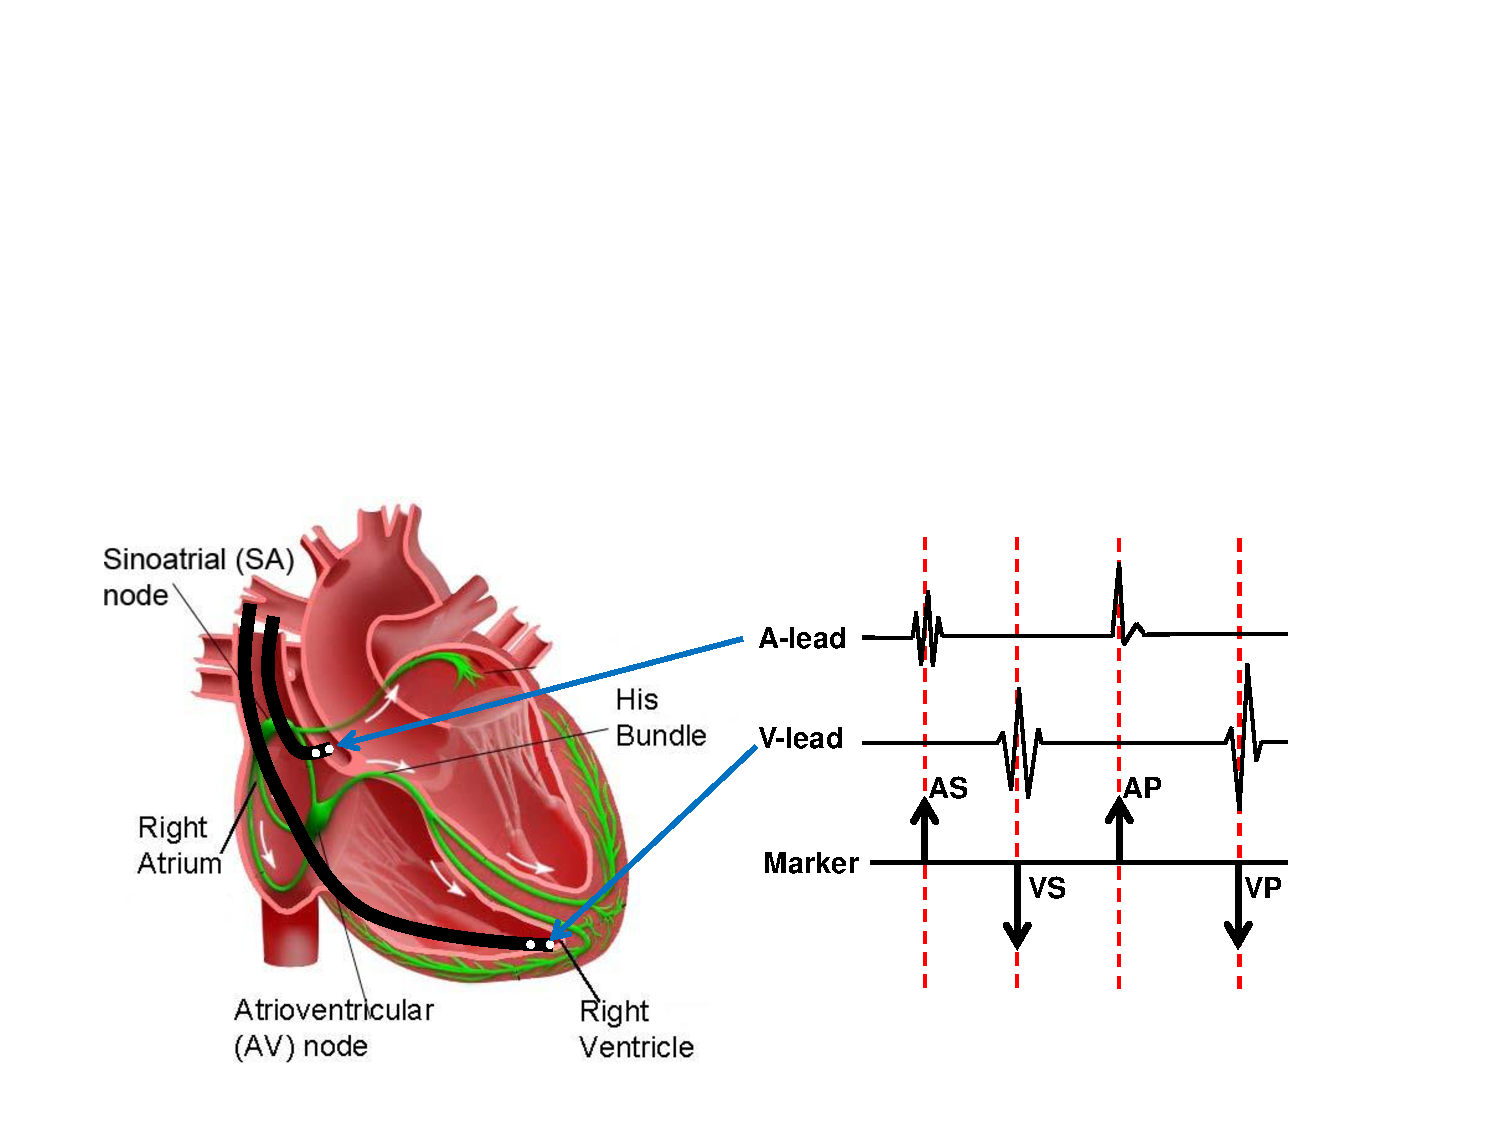
\includegraphics[width=0.9\textwidth]{figs/egm.pdf}
		
%\vspace{-10pt}
\caption{\small (a) Lead placement for a dual chamber pacemaker. (b) Electrogram (EGM) signals measured from pacemaker leads and corresponding internal pacemaker events}
\label{fig:probes}
%\vspace{-15pt}
\end{figure} 

%Implantable pacemakers follow the principle of EP testing. For a dual chamber pacemaker, two leads are inserted into the right atrium and right ventricle, respectively. The pacemaker senses the intrinsic generation and conduction of the electrical signals in the two chambers and deliver electrical pacing when the heart rate and/or atria-to-ventricles conduction interval are abnormal.
The implantable cardiac pacemakers are rhythm management devices designed to treat bradycardia. A typical dual chamber pacemaker has two leads inserted into the heart through the veins which can measure the local electrical activity of the right atrium and right ventricle respectively (\figref{probes}.a). According to the timing between sensed impulses, the pacemaker may deliver electrical pacing to the corresponding chamber to maintain proper heart rhythm.

\begin{figure}[!t]
\centering
		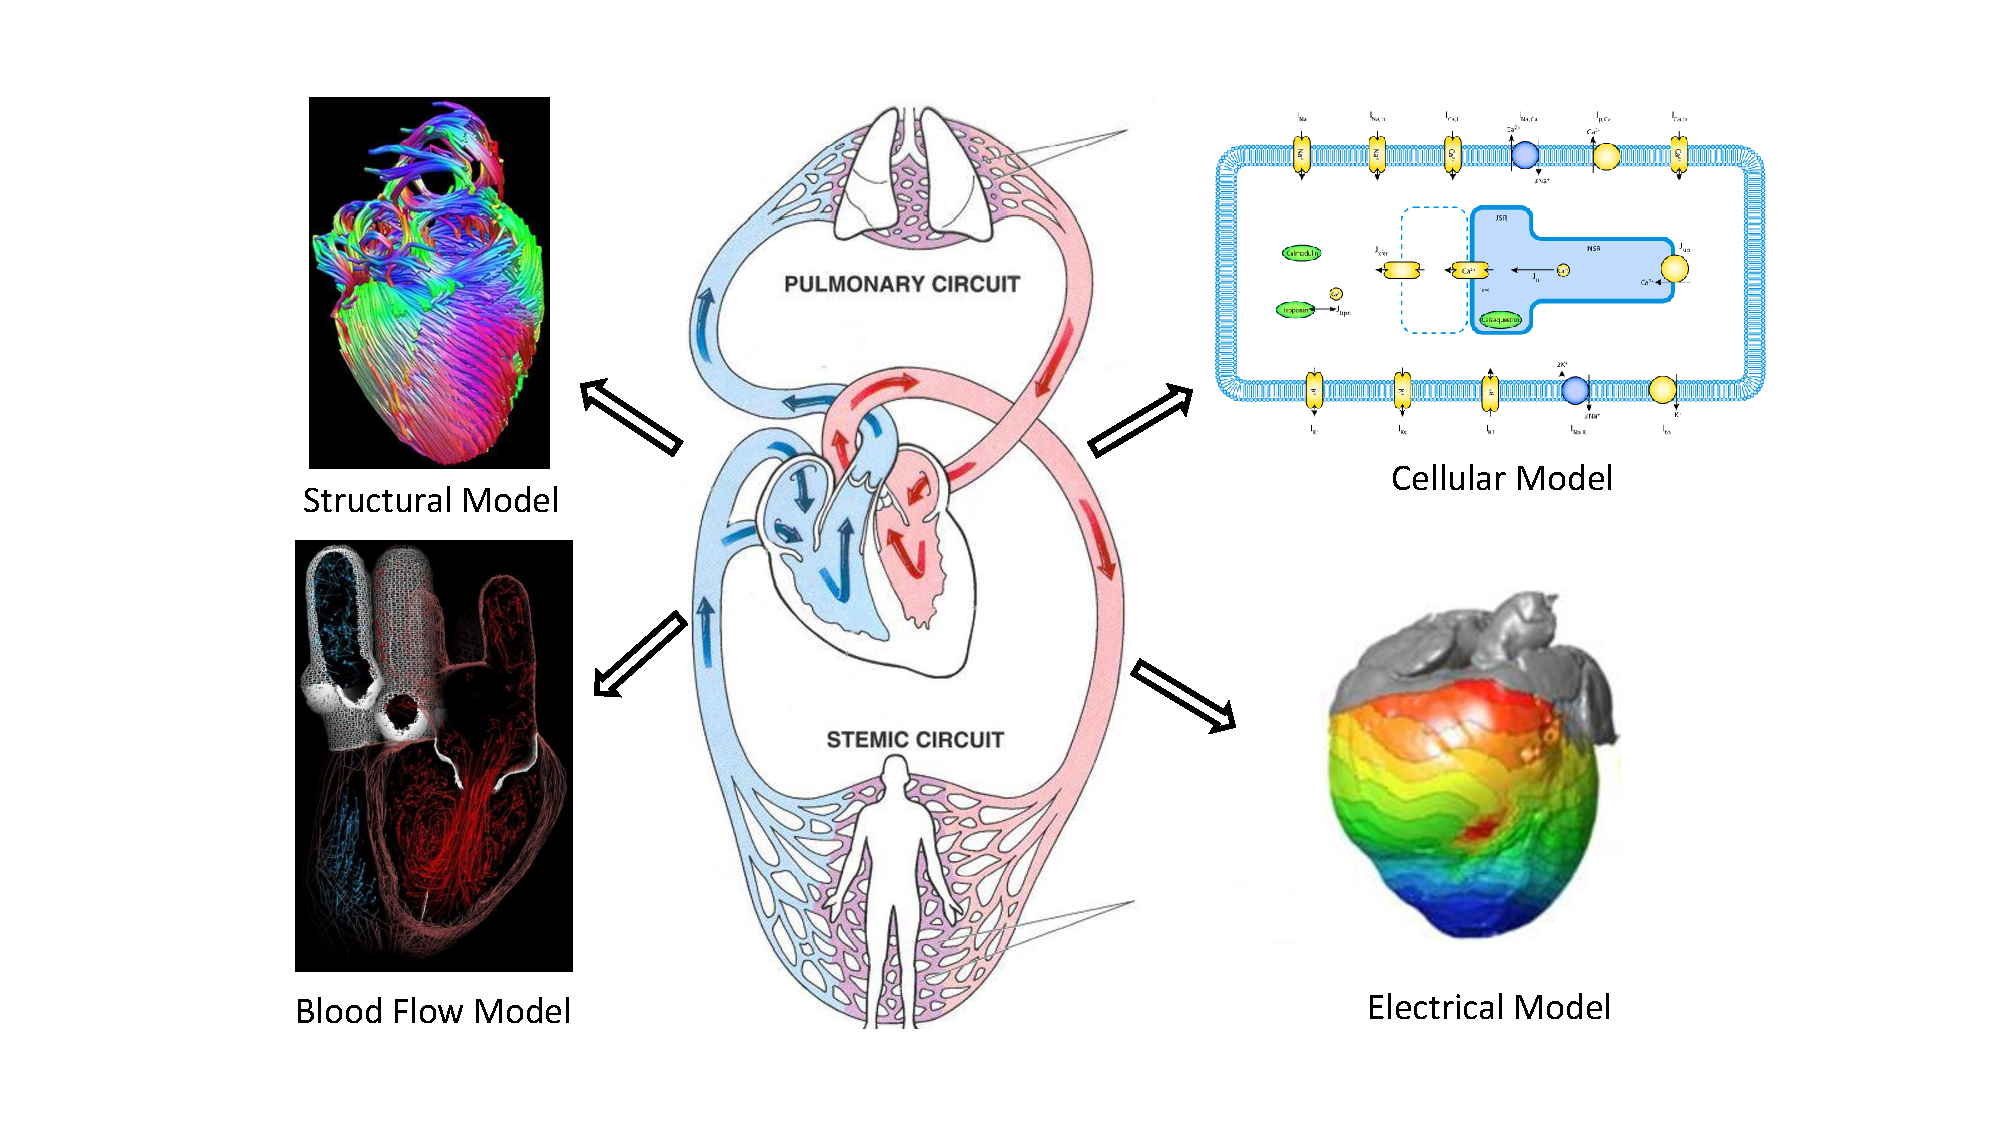
\includegraphics[width=0.9\textwidth]{figs/models.pdf}
		
%\vspace{-10pt}
\caption{\small Physiological models of the heart from different perspectives}
\label{fig:models}
%\vspace{-15pt}
\end{figure} 
\section{Physiological Models of the Heart}
To study the mechanisms of heart diseases and their effects on cardiac output, different physiological models of the heart have been developed. \figref{models} illustrates several aspects that these models capture. With the development of the imaging techniques like MRI, detailed anatomical structures of the heart can be modeled and studied (\cite{geometric}). These models are fundamental in other modeling aspects as well, as the anatomy of the heart dictates the electrical and mechanical behaviors of the heart. \figref{models}.(a) shows models for heart muscle fiber orientations by \cite{fiber}. With anatomy models the electrical and/ or mechanical properties of the heart can be studied. \figref{models}.(b) illustrate a model of blood flow within the ventricles (\cite{bloodflow}). Electrical properties of the heart at cellular level has been modeled (\cite{cellular}) and by combining these cellular models with the structural models, the electrical activities of the whole heart are studied, especially the mechanism of different arrhythmia (\cite{natalia},~\cite{Grosu_MHA},~\cite{Grosu_wave}). Intrinsic heart rate variability has been modeled to synthesize optimal control of pacemaker pacing. (\cite{Bogdan}) Abstraction of the electrical cellular model has also been attempted by \cite{Grosu_abstract} to reduce model complexity without sacrificing accuracy. The electrical properties and the mechanical properties of the heart are closely coupled. Models combining both of these aspects are also developed to study the effects of different arrhythmia on cardiac outputs (\cite{natalia},~\cite{eletro_mechanical}).

\section{Heart Models for Closed-loop Validation of   Implant-able Cardiac Devices}
Models should be developed according to their applications. The aforementioned models of the heart are mostly used for understanding the mechanisms of different heart diseases. Physiological models developed for closed-loop evaluation of medical devices should have the following considerations:\\
\textbf{C1. Interfacing with the device: }The model should be able to generate physiological signals that the device sense from the real physiological entities. And the model should be able to take device output as input and change its states accordingly. Model complexity should also be adjusted according to the device interface to hide unnecessary details.\\
\textbf{C2. Differentiate different physiological conditions: }To evaluate the safety and effectiveness of the device, the device has to be evaluated under certain physiological conditions specified by the requirements. For example, the pacemaker is supposed to maintain proper heart rate during Bradycardia. The model should be expressive enough to be able to differentiate the physiological condition (Bradycardia in the example) from other conditions. Failing to do so may result in false-positives or false-negatives in the evaluation result. \\
\textbf{C3. Physiological/logical interpretation of model states: } In closed-loop evaluation we are checking the device safety and effectiveness against the physiological requirements. However, due to the limited interface (e..g two leads for a dual chamber pacemaker) it is always difficult to determine only from an execution trace that the therapy is safe and effective. Therefore, being able to provide physiological meanings to the states of the model also allows us to interpret the closed-loop execution more accurately, thus reducing the number of physiologically impossible executions during the evaluation. To satisfy these requirements, the model structure of these physiological models should base on physiological or clinical first principles so that states and state transitions of the closed-loop executions can be explained with physiological language. \\%One advantage of closed-loop evaluation over open-loop evaluation is the capability to provide physiological/logical interpretation of an execution trace. With this advantage we are able to identify and reduce the number of physiological-impossible executions by examining the state of the model, so that the evaluation can focus on physiological-possible executions. This requires the model first-principle\\
\textbf{C4. Available patient data: } In closed-loop evaluation, physiological models are developed to represent certain physiological condition across a population of patients or even a particular patient. The model parameters must be identified so that the behaviors of the models match the behaviors of the patients (groups).  Due to the limited sensing capability of closed-loop medical devices, the obtained data is sparse. i.e. we can not put a sensor on every tissue region of the heart. Therefore the complexity of the model should be in accordance with the available data to avoid \emph{over-fitting}, which occurs when a model has too many parameters relative to the number of observations, and this can introduce errors during prediction. 

The electrophysiological models mentioned in the last section (\cite{natalia,Grosu_MHA}) satisfy C1-C3. However, the parameter space of these models are too large (10+ parameters for each cellular model multiplied by $10^5$ of elements) which not only increase simulation complexity, but also impossible to identify due to lack of data. As introduced in Section \ref{EP}, the pacemaker has only two leads at fixed locations and only use timing between local activation events for diagnosis. These models with high spatial fidelity possess details that can be abstracted without sacrificing the three considerations.

Electrophysiology testing (EP testing) has been an active clinical field to diagnose and treat arrhythmia with minimal-invasive procedures. During an EP testing procedure, the physicians diagnose heart conditions by examining the patterns and intervals of local electrical activations (temporal) measured from electrodes placed into different locations of the heart (spatial). EP testing is the perfect modeling level for closed-loop evaluation of implantable cardiac devices because: 1) it is the basis of implantable cardiac devices (C1), 2) physicians can use EP testing to diagnose most arrhythmia thus distinguish them (C2,C3), 3) there are abundant patient data available (C4). 

In the remaining chapter we will introduce our heart modeling efforts based on EP testing, and model adaptation for two different applications of closed-loop evaluation of implantable cardiac devices.
%\section{Heart Models for Pacemaker Interaction}
%The heart generates electrical impulses to maintain the heart rate appropriate for the physiological needs. These impulses conduct through the heart, triggering coordinated muscle contractions which pumps blood to the rest of the body. The underlying pattern and timing of these impulses determines the heart's rhythm and is key to proper heart function. Derangements in this rhythm are referred to as \emph{arrhythmia}, which 



%\subsection{Electrical conduction system of the heart}
%Heart tissue with different timing parameters form the electrical conduction system to ensure coordinated contraction of the heart. First, specialized tissue at the Sinoatrial (SA) node periodically and spontaneously self-depolarizes. This is controlled by the nervous system and the SA node is the primary and natural pacemaker of the heart. The activation signal then travels through both atria, causing contraction and pushes blood into the ventricles. Then the activation is delayed at the Atrioventricular (AV) node which allows the ventricles to fill fully. The fast-conducting His-Purkinje system then spreads the activation signal within both the ventricles. The simultaneous contraction of the ventricle muscles will push the blood out of the heart.
%\begin{figure*}[!t]
%\centering
		%\subfigure [\small]{			
		%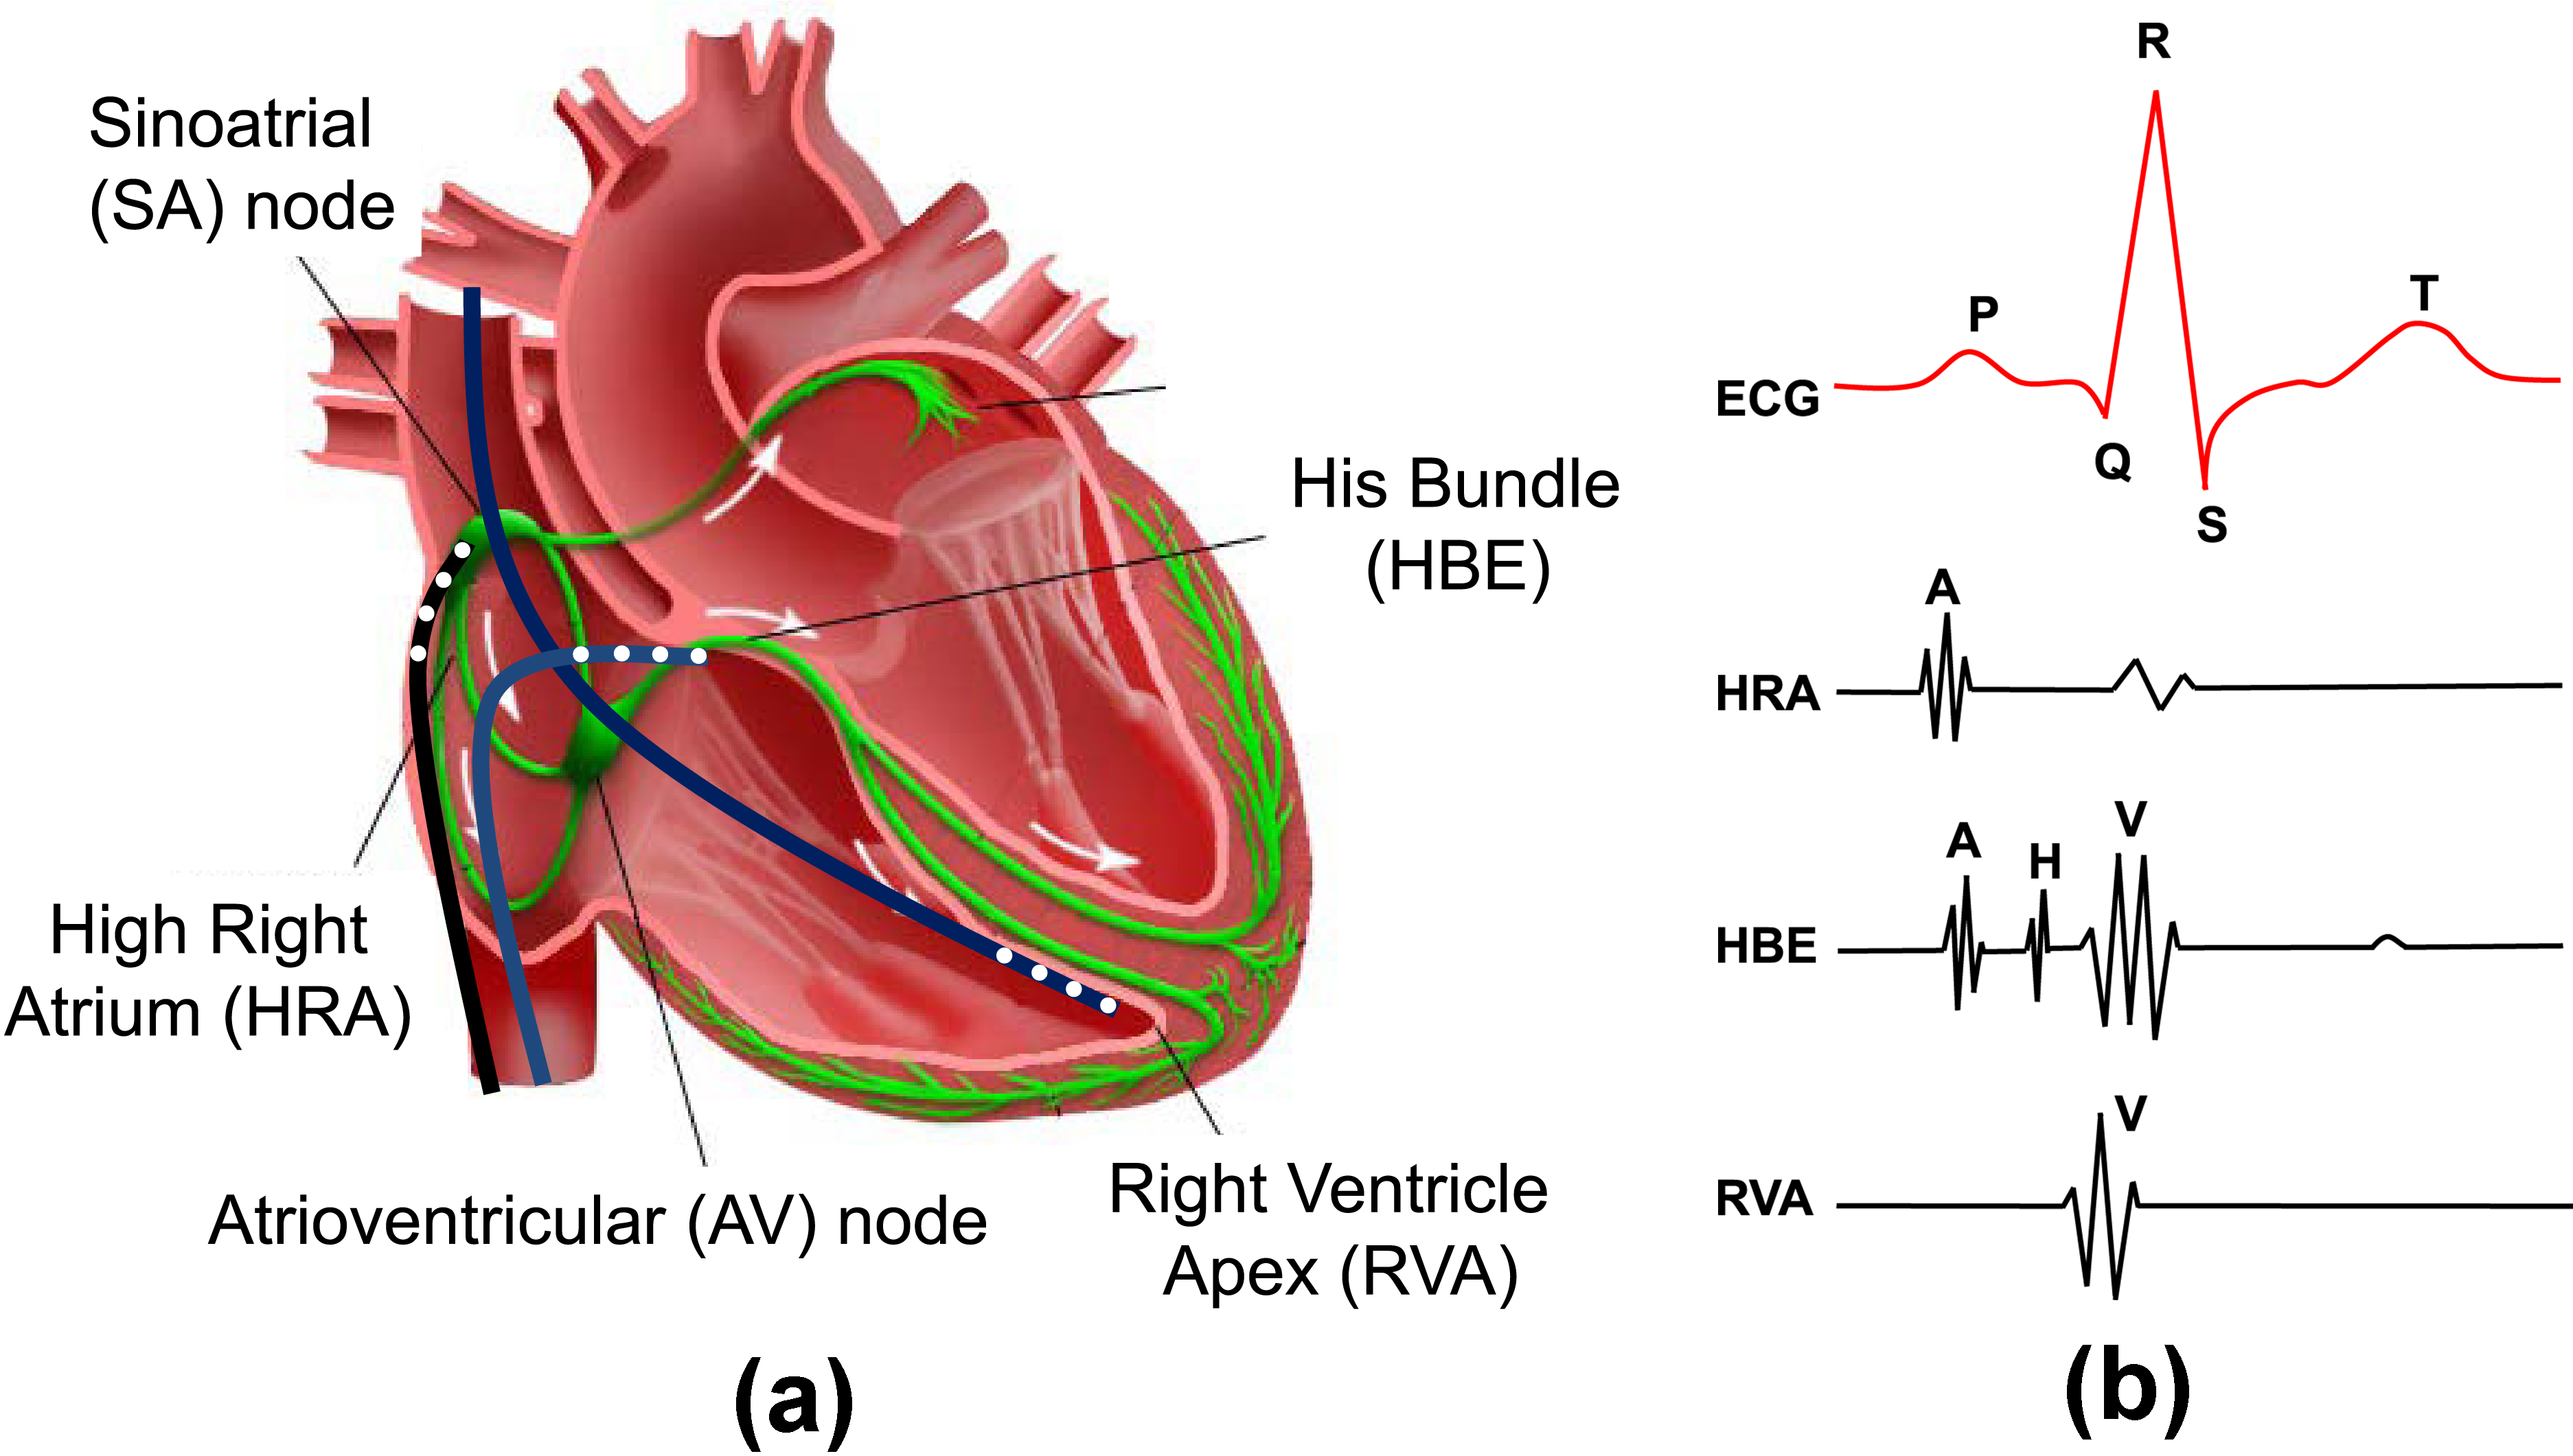
\includegraphics[width=0.3  \textwidth]{figs/probes.png}
		%\label{fig:probes}
		%} 
%
		%\subfigure [\small] 
		%{
		%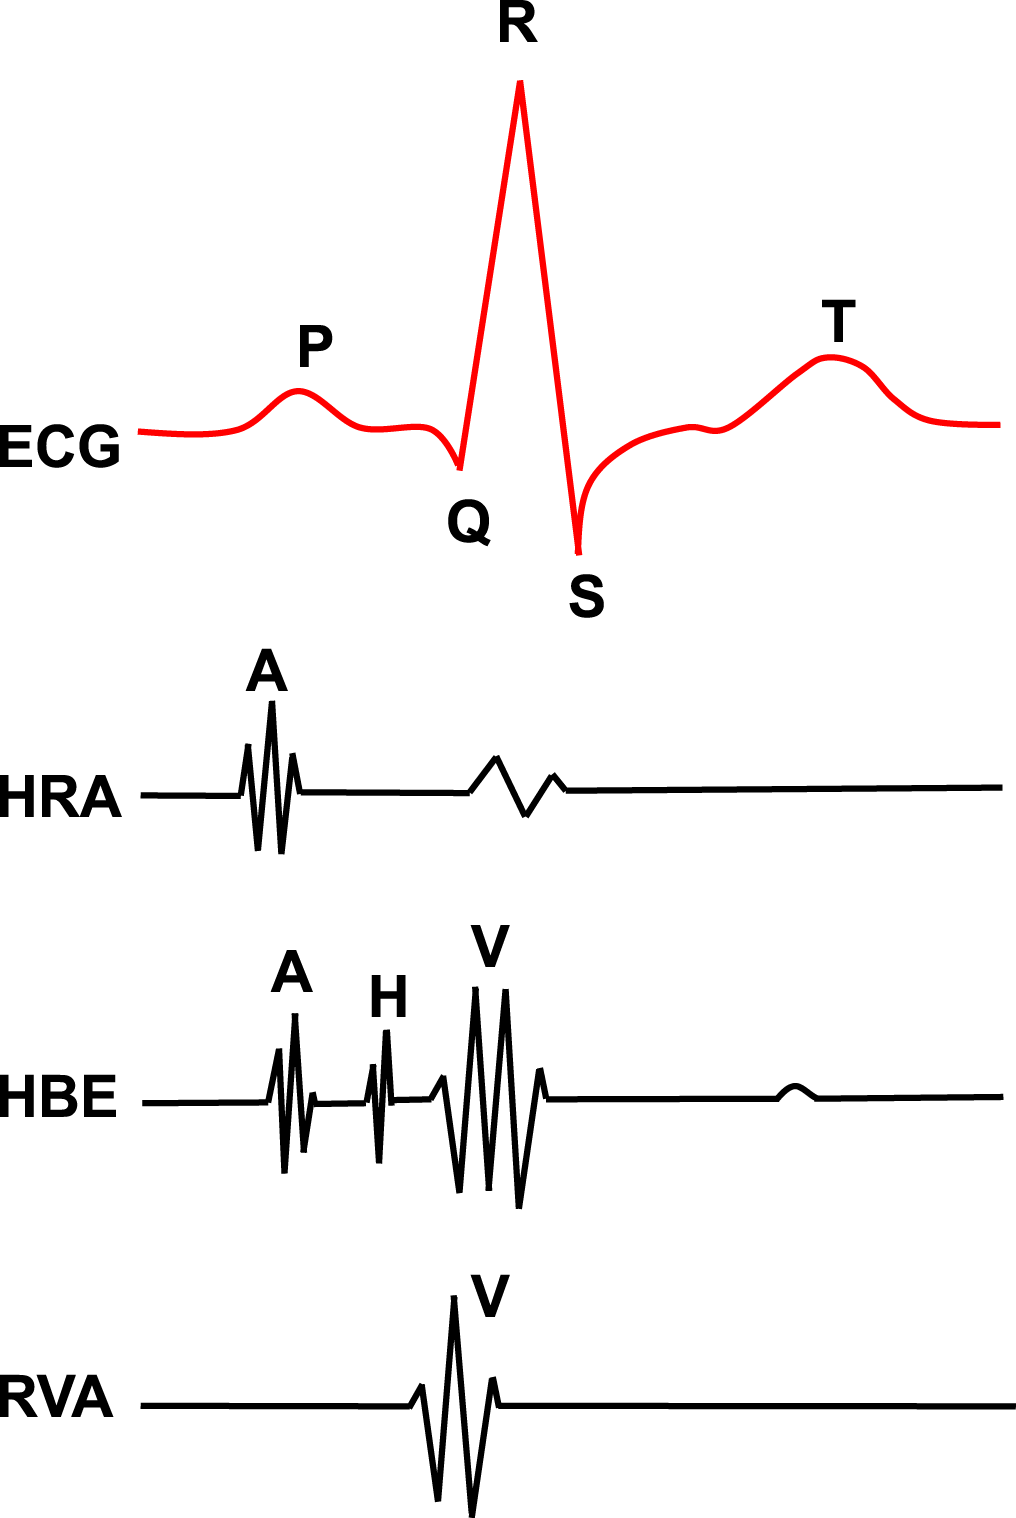
\includegraphics[width=0.2\textwidth]{figs/egm.png}
		%\label{fig:egm}
		%} 
%%\vspace{-10pt}
%\caption{\small (a) Node automaton. Dotted transition is only valid for pacemaker tissue like SA node; (b) Path automaton; (c) Model of the electrical conduction system of the heart using a network of node \& path automata~\cite{vhm_ecrts10}.}
%%\vspace{-15pt}
%\end{figure*} 

%\section{Electrophysiological Testing}
%\Hao{A figure for heart and pacemaker}

%\chapter{Modeling the Physiological Environment}
%\begin{itemize}
	%\item How to encode domain knowledge of the physiological environment into models?
    %\item What are the applications that the models will be used?
    %\item What are the differences in terms of environment models between model checking and simulation?
    %\item How to balance complexity and expressiveness of the model?
%\end{itemize}

%In the following sections, we demonstrate how to construct heart models for closed-loop verification of implantable pacemaker. Note that for two different applications the models are constructed differently as we address their respective requirements for environment models. 


\section{Heart Models for Closed-loop Testing}
%\begin{itemize}
	%\item Why the models at this level have to be deterministic? Where can they be used?
    %\item How electrophysiology reflects the functions of the heart?
    %\item How to encode these knowledge into models?
    %\item Why VHM has the right level of details for pacemaker verification?
    %\item How VHM interacts with pacemaker?
    %
%\end{itemize}
During closed-loop testing, the devices interact with the environment (or its models) under different environmental conditions. The closed-loop executions are monitored and violations of safety and efficacy requirements are reported. In model-based closed-loop testing, the environment models are expected to mimic the behaviors of actual environment and its interaction with the device. Thus, the environment models are in general deterministic so that the execution traces are reproducible and are able to mimic different arrhythmia. Complex dynamics during state transitions also need to be captured to validate violations within longer executions traces. 

\subsection{Modeling Philosophy}
As the pacemaker can only sense and actuate from two locations within the heart, only structures and parameters that affect inputs to the pacemaker are needed. Since the two leads are fixed, the accurate spatial locations of different heart anatomical structures are not necessary. Instead, the topology of the electrical conduction system of the heart is more important. 


\begin{figure}[!t]
\center
%\vspace{-10pt}
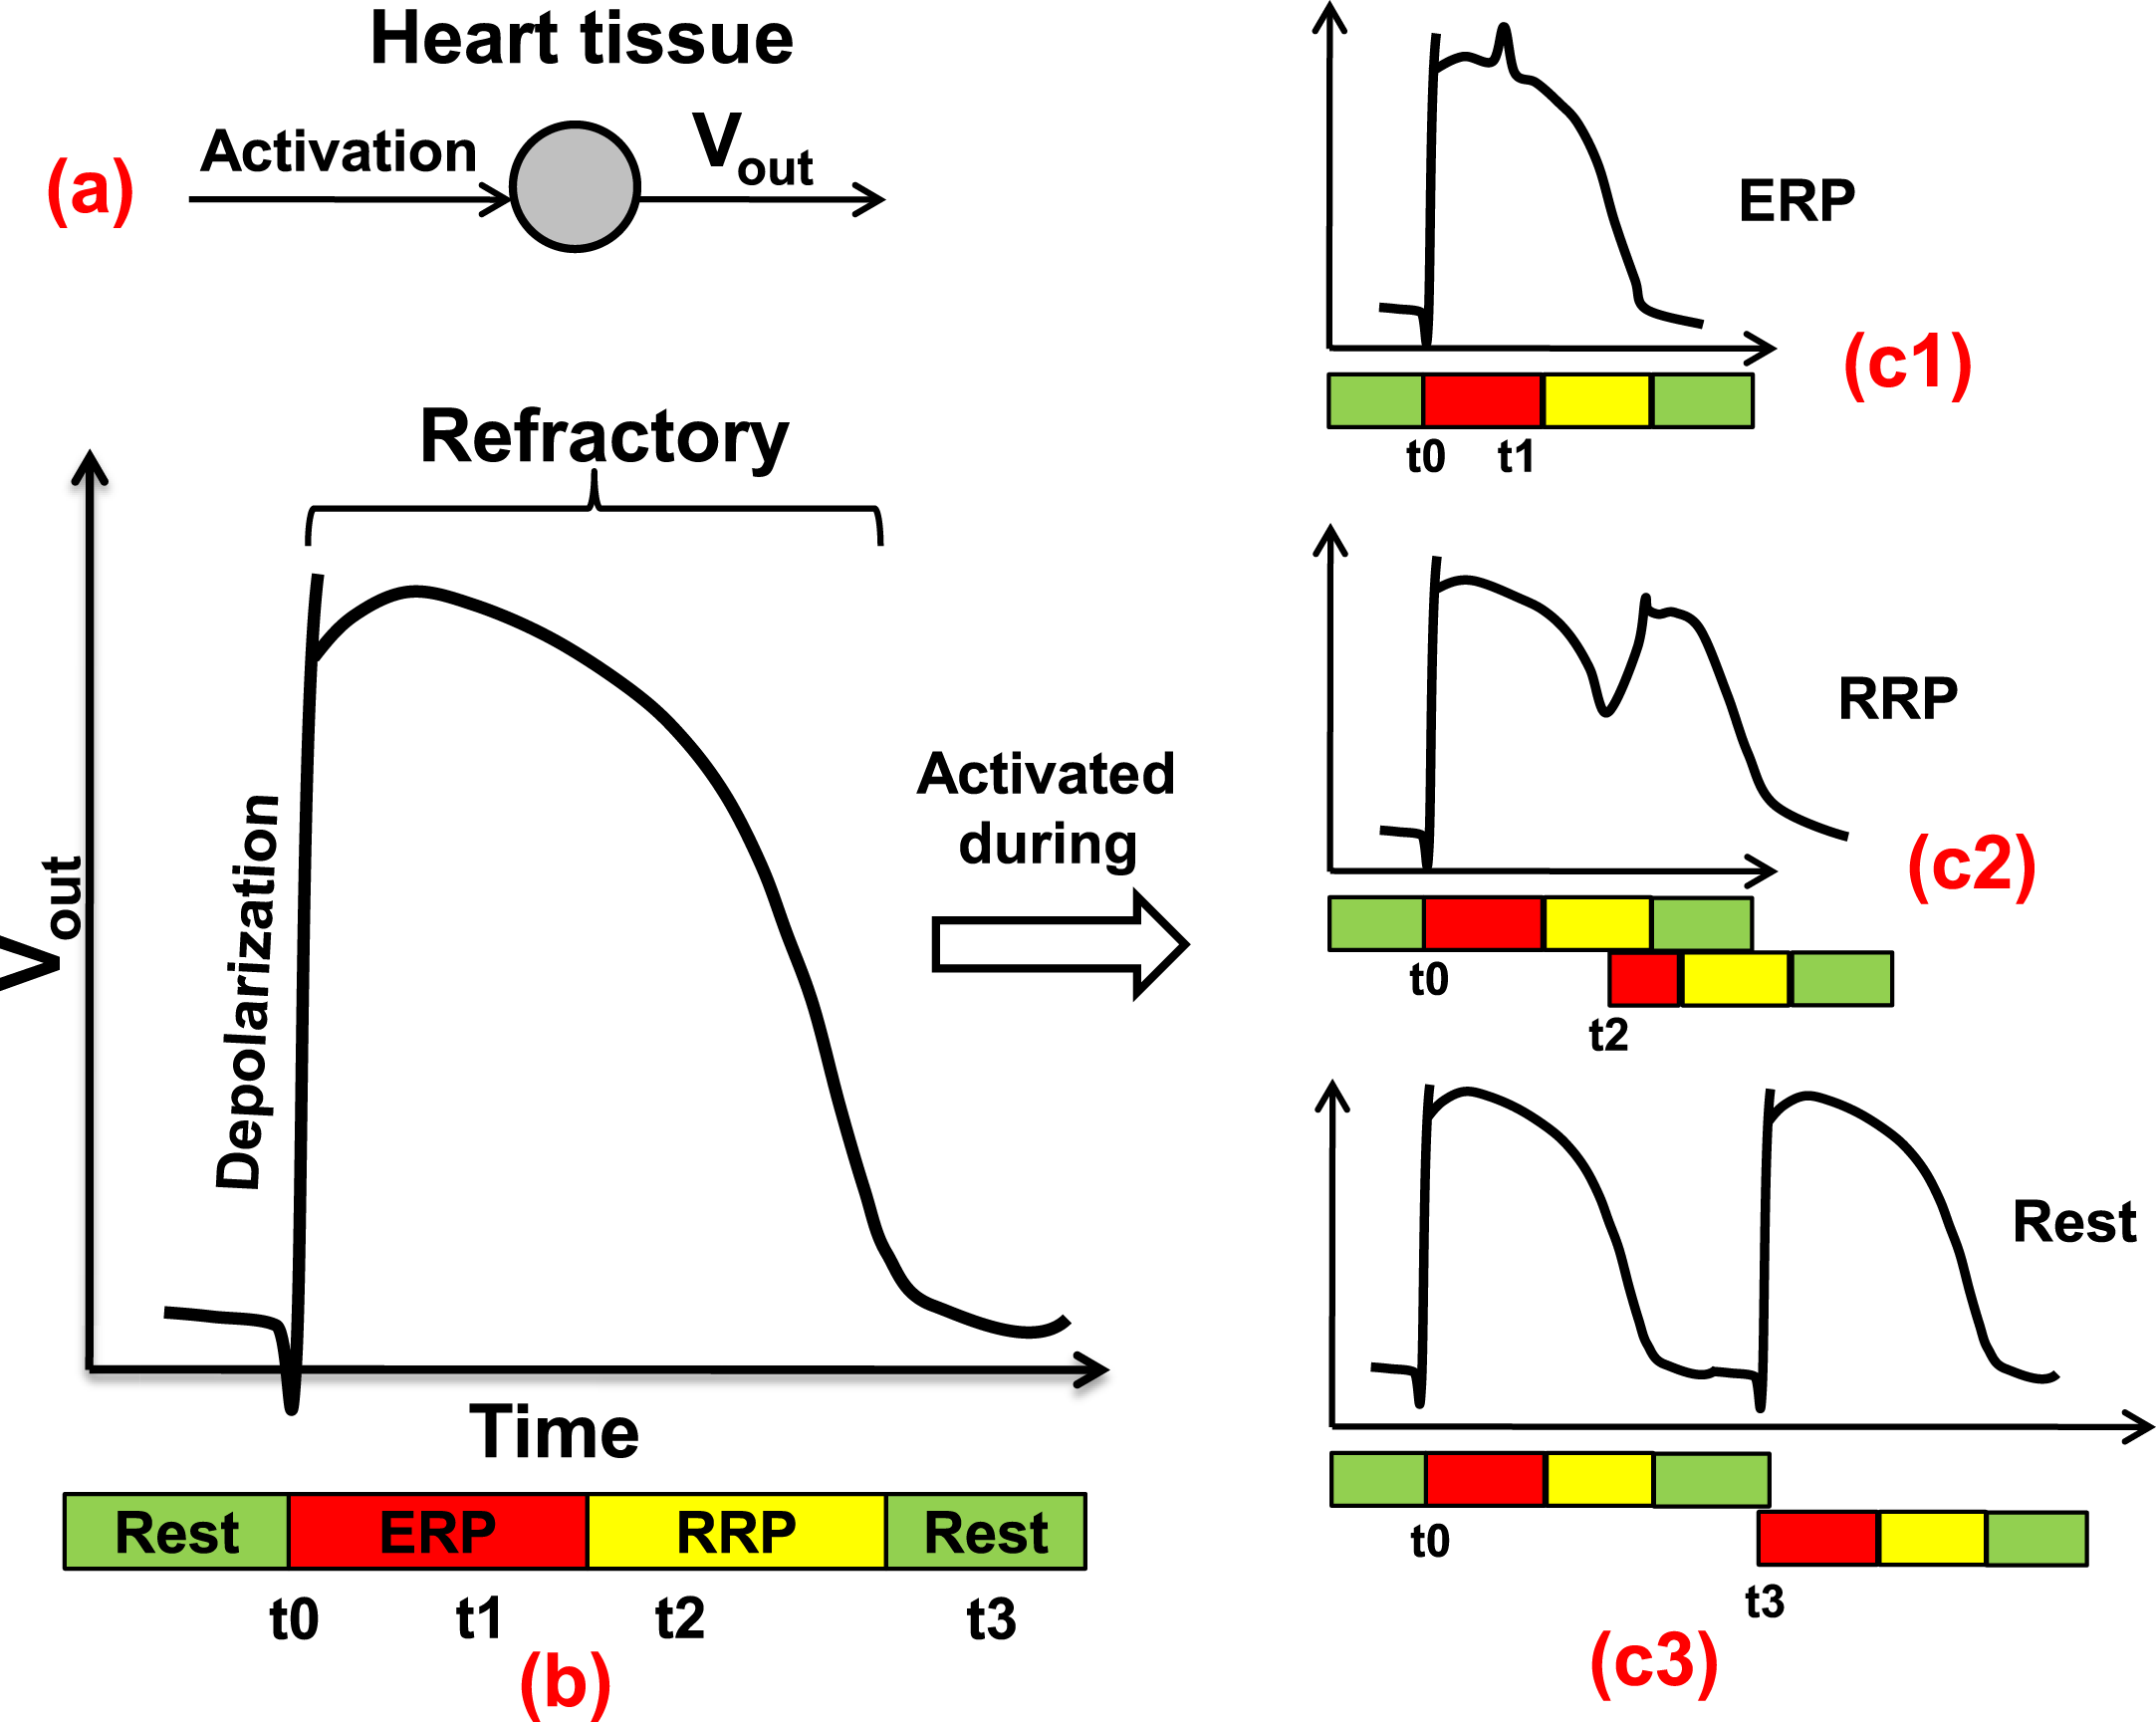
\includegraphics[width=0.7\textwidth]{figs/refractory.png}
%\vspace{-10pt}
\caption{(a) The generation of Action potential; (b) Action potential; (c1) The second activation arrived during ERP; (c2) Arrived during RRP; (c3) Arrived after refractory.}
\label{fig:refractory}
%\vspace{-10pt}
\end{figure} 
\subsection{Timing Behaviors of Cellular Electrophysiology}
The contraction of heart muscles is triggered by external voltage applied to the tissue. After the activation, a transmembrane voltage change over time can be sensed due to ion channel activities, which is referred to as an Action Potential (\figref{refractory}(a)). The upstroke of the action potential is called depolarization, during which the muscle will contract. The voltage change caused by the depolarization will depolarize the tissue nearby, which causes an activation wave across the heart. After the depolarization there is a refractory period during which the tissue recovers to the pre-excitation state and the voltage drops down to the resting potential. The refractory period can be divided into \emph{Effective Refractory Period (ERP)} and \emph{Relative Refractory Period (RRP)} (\figref{refractory}(b)). During ERP, the tissue cannot be depolarized due to the lack of charge. As a result, the activation wave will be "blocked" at the tissue during ERP (\figref{refractory}(c1)). During RRP, the tissue is partially recovered and the tissue can be depolarized. However, the new action potential generated by the depolarization will have different morphology (e.g. attenuated in magnitude and duration), thus affecting the refractory periods of the tissue and conduction delay of the activation wave (\figref{refractory}(c2)). \figref{refractory}(c1)-(c3) show the action potential shape change and corresponding timing change in refractory periods when the tissue is activated at time stamp $t1$, $t2$, $t3$ after the initial activation $t0$. 

\subsection{Heart Model Components}
We introduce the model components that can be used to configure heart models corresponding to different heart conditions. As discussed earlier, the action potential of a heart tissue has 3 timing periods during which the tissue responds to external electrical stimuli differently. We use an extended timed-automata formulation (\cite{timed_automata}) to model the timing behaviors of a heart tissue during each cycle. 

\textbf{Node Automata:} We refer to the tissue model as \emph{node automaton} and \figref{automata}.(a) shows the structure of a node automaton $i$. 3 states correspond to the timing periods of the action potential. From \textsf{Rest} state, the node can either self-activate or get activated by external stimuli (Act\_node) and go to \textsf{ERP} state. During \textsf{ERP} state the node does not respond to external stimuli (blocked). During \textsf{RRP} state, the node can still be activated and go to \textsf{ERP} state, however the ERP period and the conduction delay of the tissue are affected by the "earliness" of the activation arrived during the RRP period, which is tracked by a shared variable $C(i)$. The new ERP period is determined by a function over clock value $g(f(t))$ which mimics the beat-to-beat dynamics described in \cite{josephson}. The function $g$ and $f$ are given by:
\begin{equation} \label{factor}
						f(t) = 1-t/Trrp
						\end{equation}
and
%  The AV node has a different profile than the other tissue. The ERP period increases rather than decreases when activated during its RRP (~\cite{josephson}).
\begin{equation} \label{earliness_noAV}
						g(x) = \left\{
						\begin{array}{lr}
						
						T_{min}+(1-(1-x)^3)\cdot (T_{max}-T_{min}), i=AV\\
						T_{min}+(1-x^3)\cdot (T_{max}-T_{min}),i\neq AV
			
						
						\end{array}
						\right.
						\end{equation}  
where $T_{min}$ and $T_{max}$ are the minimum and maximum value for \emph{Terp} of the tissue.
\begin{figure}[!t]
%\centering
		%\subfigure [\small]{			
		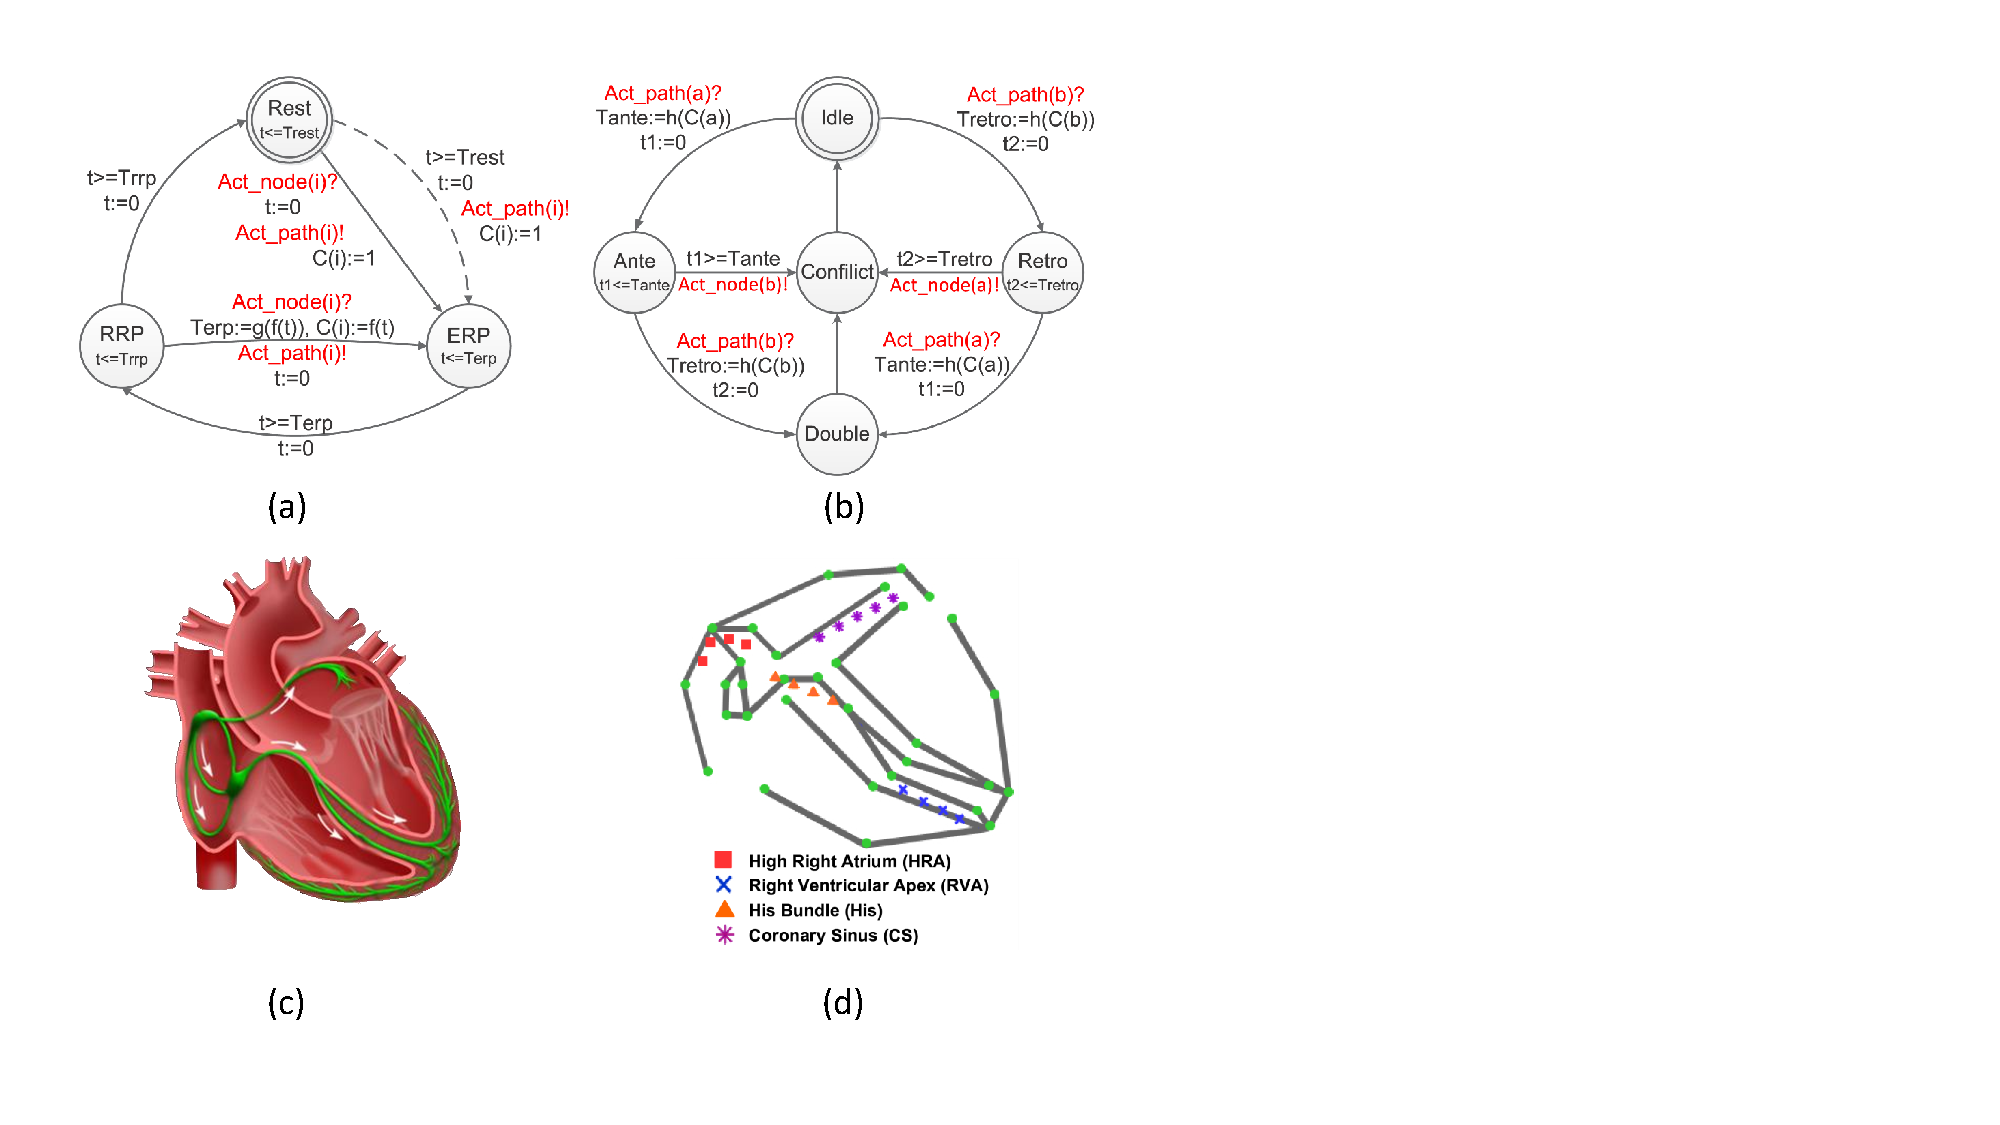
\includegraphics[width=1.2\textwidth]{figs/automata.pdf}
		%\label{fig:node_automata}
		%} 
%%	\hspace{.1in}%
		%\subfigure [\small] 
		%{
		%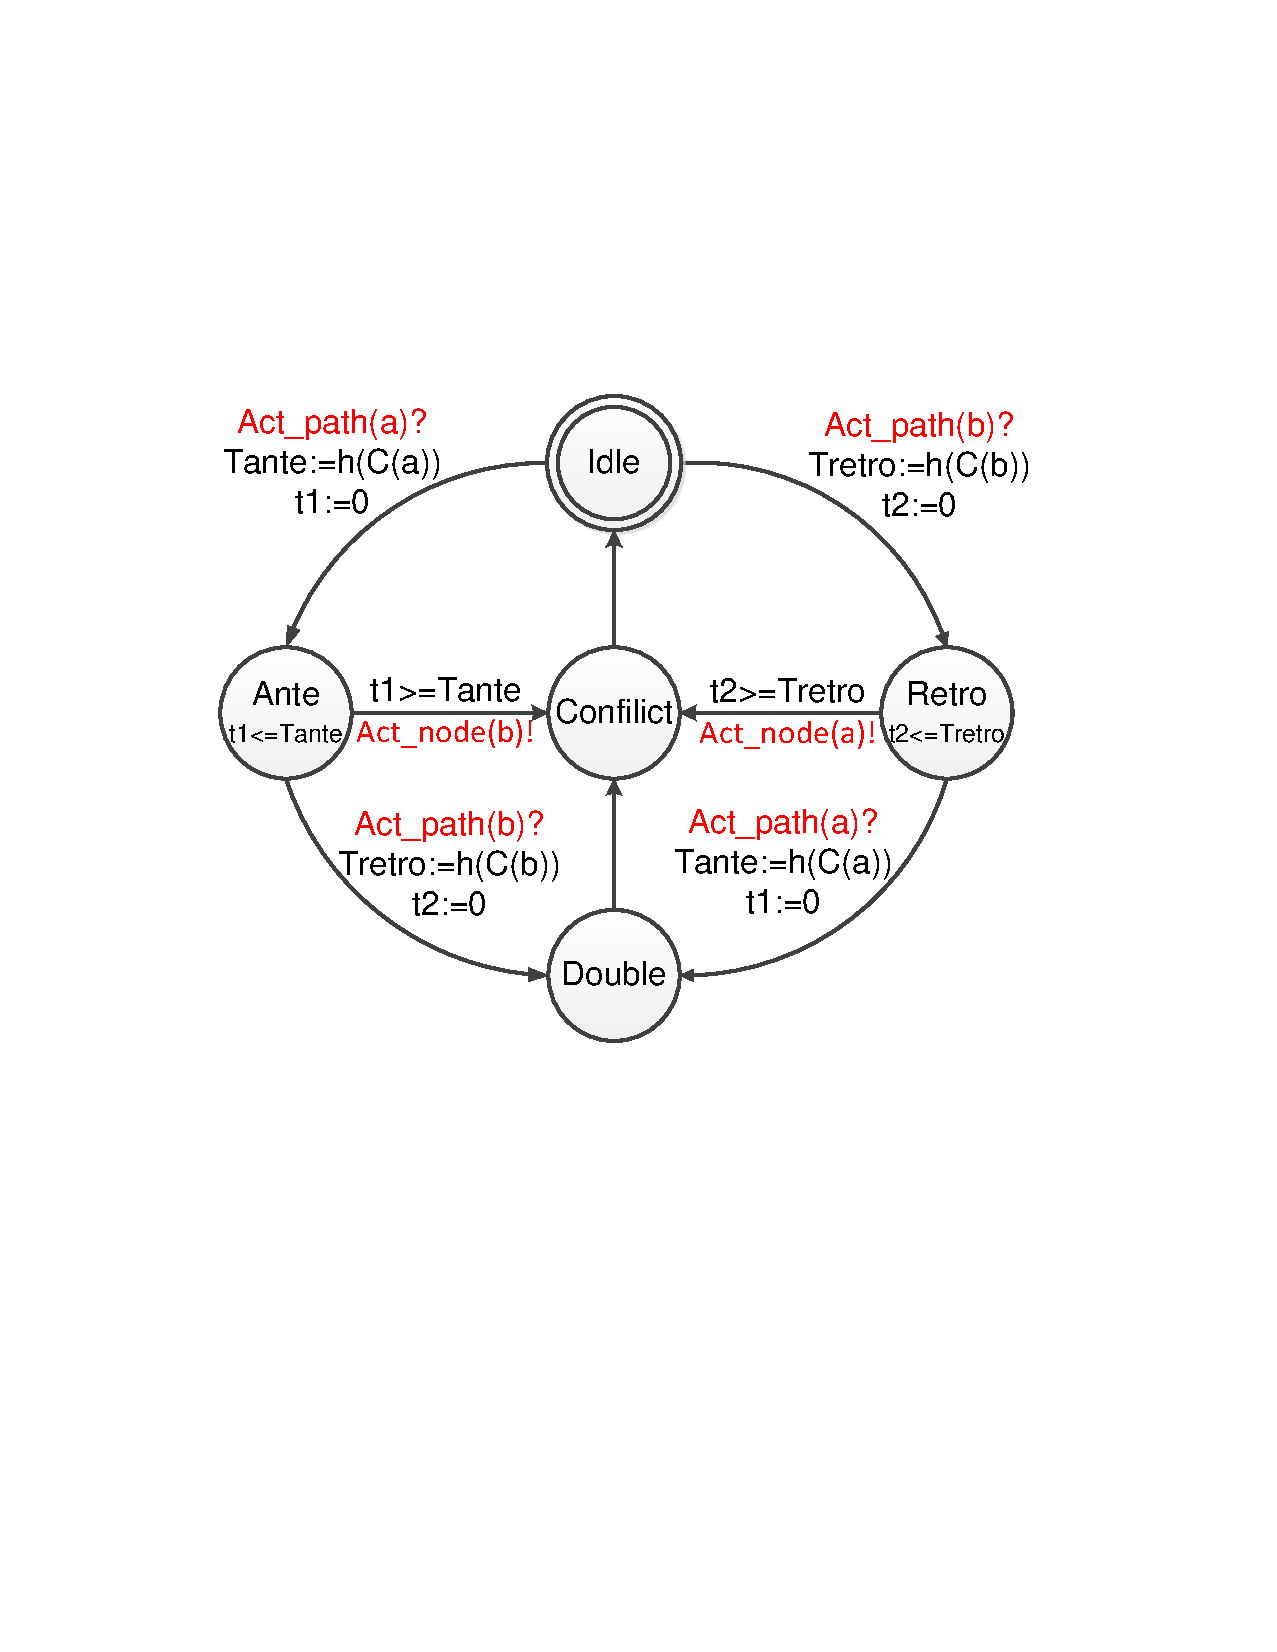
\includegraphics[width=0.32\textwidth]{figs/path.pdf}
		%\label{fig:path_automata}
		%} 
		%\subfigure [\small] 
		%{
		%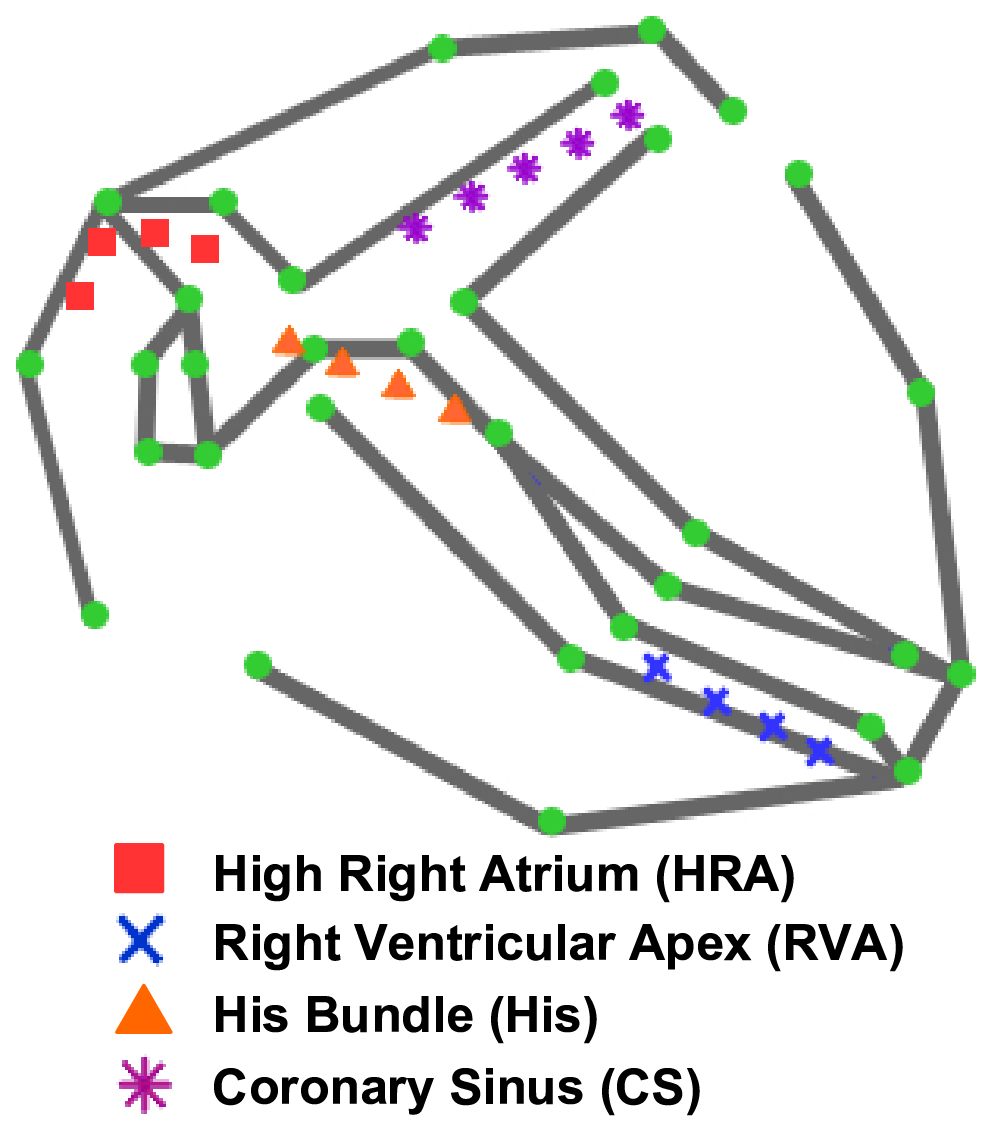
\includegraphics[width=0.25\textwidth]{figs/gen_setup.png}
		%\label{fig:general_setup}
		%} 

%\vspace{-10pt}
\caption{\small (a) Node automaton: The dotted transition is only valid for tissue (like SA node) that can be activated by an external trigger; (b) Path automaton modeling the electric conduction and propagation between two node automata; (c) Model of the electrical conduction system of the heart using a network of node \& path automata ~\cite{VHM_proc}.}\label{fig:automata}
%\vspace{-15pt}
\end{figure} 

Due to the limited number of observable points within the heart, modeling the electrophysiological behavior of every tissue of the heart and its full anatomy is unnecessary and unfeasible. In our heart models, only self-activating tissue and key hubs of the electrical conduction system are modeled as node automata. 

\textbf{Path Automata:} The electrical conduction through the tissue between nodes are abstracted using \emph{path automata}. The path automata can be used to represent structural or topological (functional) electrical connections between nodes. \figref{automata}.(b) shows a path automaton connecting node a and b.

The initial state of a path automaton is \emph{Idle}, which corresponds to no conduction. The states corresponding to the two conduction directions are named after the physiological terms: Antegrade (Ante) and Retrograde (Retro). These states can be intuitively described as forward and backward conductions. If path actuation \emph{Act\_path} event is received from one of the nodes connected to it, there is a transition to \emph{Ante} or \emph{Retro} state based on the activation source in the path automaton. At the same time, the clock invariant of the state is modified according to the shared variable \emph{C(a/b)}. This corresponds to the change of the conduction delay that is caused by the early activation. Similar to node automaton, the changing trend is extracted from clinical data and the function $h$ is defined as:
\begin{equation} 
						h(c) = \left\{
						\begin{array}{lr}
						
						path\_len/v\cdot (1+3c), i=AV\\
						path\_len/v\cdot (1+3c^2), i\neq AV
						\end{array}
						\right.
						\end{equation}
where $path\_len$ denotes the length of the path and $v$ is the conduction velocity.

After \emph{Tante} or \emph{Tretro} time expires, the path automaton sends out \emph{Act\_node(b)} or \emph{Act\_node(a)} respectively. A transition to \emph{Conflict} state occurs followed by the transition to \emph{Idle} state. The intermediate state \emph{Conflict} is designed to prevent back-flow, where the path is activated by the node \emph{b} it has just activated. If during \emph{Ante} or \emph{Retro} state another \emph{Act\_path} event is received from the other node connected to the path automaton, a transition to \emph{Double} state will occur, corresponding to the two-way conduction. In this case, the activation signals eventually cancel each other and the transition to \emph{Idle} state is taken.

\subsection{Modeling the Heart's Electrical Conduction System}
The node and path automata are the basic building blocks for heart modeling. Hearts with different conditions are modeled by using different conduction topologies with appropriate timing parameters for each node and path automata. \figref{automata}.(c) shows one such  topology of a network of node and path automata.

\subsection{Interaction with the Heart Model}
In EP testing and during pacemaker implantation, the local electrical activities, measured as electrogram (EGM) signals, are used to diagnose heart conditions. During heart model construction, we can assign a node automaton at electrode locations and the transitions to the ERP state can be used to represent the local activation events. In a more general setup where electrodes are assigned anywhere within the heart model, a probe model is designed to generate synthetic EGM signals using spatio-temporal information from the proximity to the network of node and path automata. \figref{egm_s} shows the morphology of EGM signal changes with different conduction velocity and probe configurations. A detailed description of the probe model can be found in \cite{vhm_embc11}.

\begin{figure}[!t]
\center
%\vspace{-15pt}
		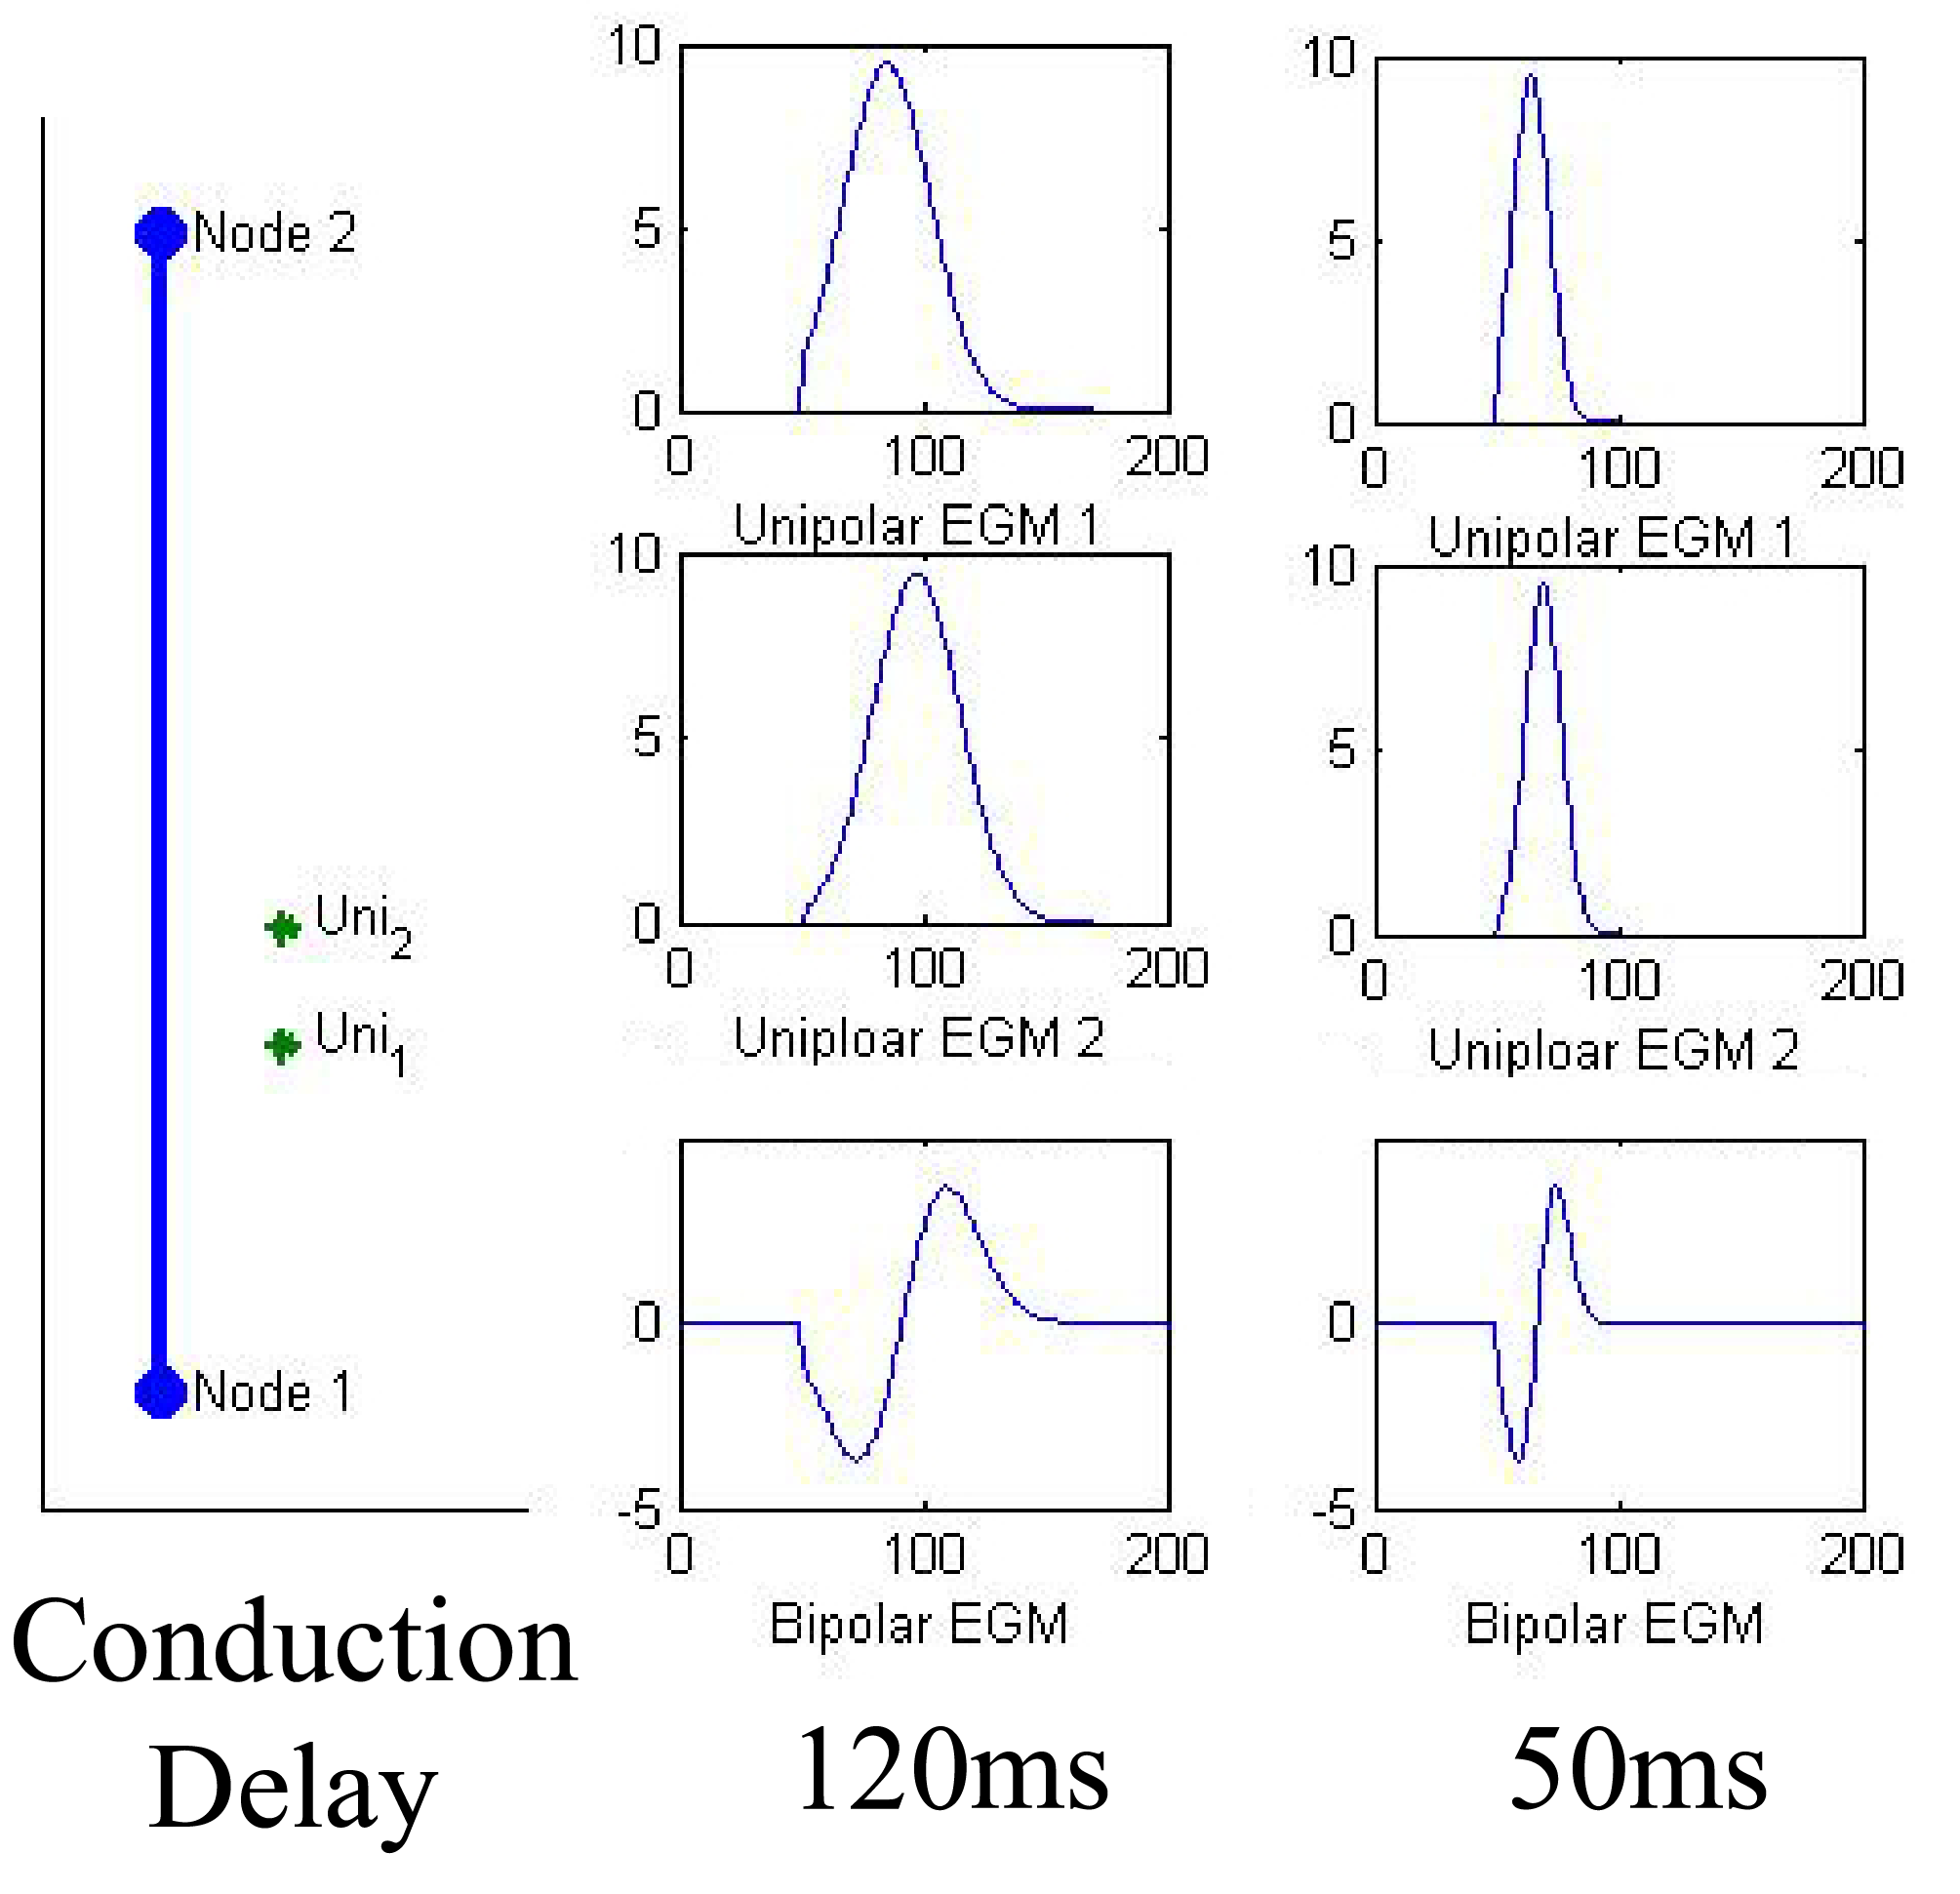
\includegraphics[width=0.7\textwidth]{figs/fig7.png}
%\vspace{-10pt}
\caption{The influence of conduction velocity and probe configuration on the EGM morphology. The left columns show the placement of probes in relation to the path; the right columns show the functional EGM.}
\label{fig:egm_s}
%\vspace{-15pt}
\end{figure}
\subsection{Heart-on-a-Chip Platform}
Platform testing remains the primary means to verify and validate device software. Currently testing is done by feeding recorded open-loop heart signals to the device and evaluating the device output. Consequently, the change in the state of the heart condition, in response to device output, is not taken into account. Thus, device malfunctions involving state changes due to multiple closed-loop interactions will not be captured during open-loop testing. 

To this effect, the heart model described above is also implemented on hardware platform (\figref{modeling_heart}) for closed-loop testing. Since each heart model is a network of node and path automata running concurrently, we implemented the heart model on an FPGA, so that increasing in the number of nodes and paths would not affect real-time constraints. The second generation heart model implementation has been implemented on a lower cost fast micro-controller platform. The fast clock ensures that executions of all nodes and paths can be finished within 1ms. The Heart-on-a-Chip platform includes a heart model implementation which is able to represent common heart conditions such as bradycardia, tachycardia, heart block, etc (for mode details refer to \cite{VHM_proc}). The parameters of the heart model can be changed at run-time by either switching among pre-defined parameter sets, or sending values directly to the model through a user interface in Matlab. A monitoring system observes logical interactions between heart model and the pacemaker and checks them against safety invariants at run-time. 

As shown in (\figref{HOC}), with an analog interface the heart model can interact with a commercial pacemaker in real time. Our analog interface uses an optical isolation circuit to separate the pacemaker circuit and the heart implementation. Signals generated from the heart are attenuated to the appropriate level to interact with a Boston Scientific pacemaker and analog pacing signals are converted to pacing events received by the heart model. 
\begin{figure}[!t]
\center
%\vspace{-15pt}
		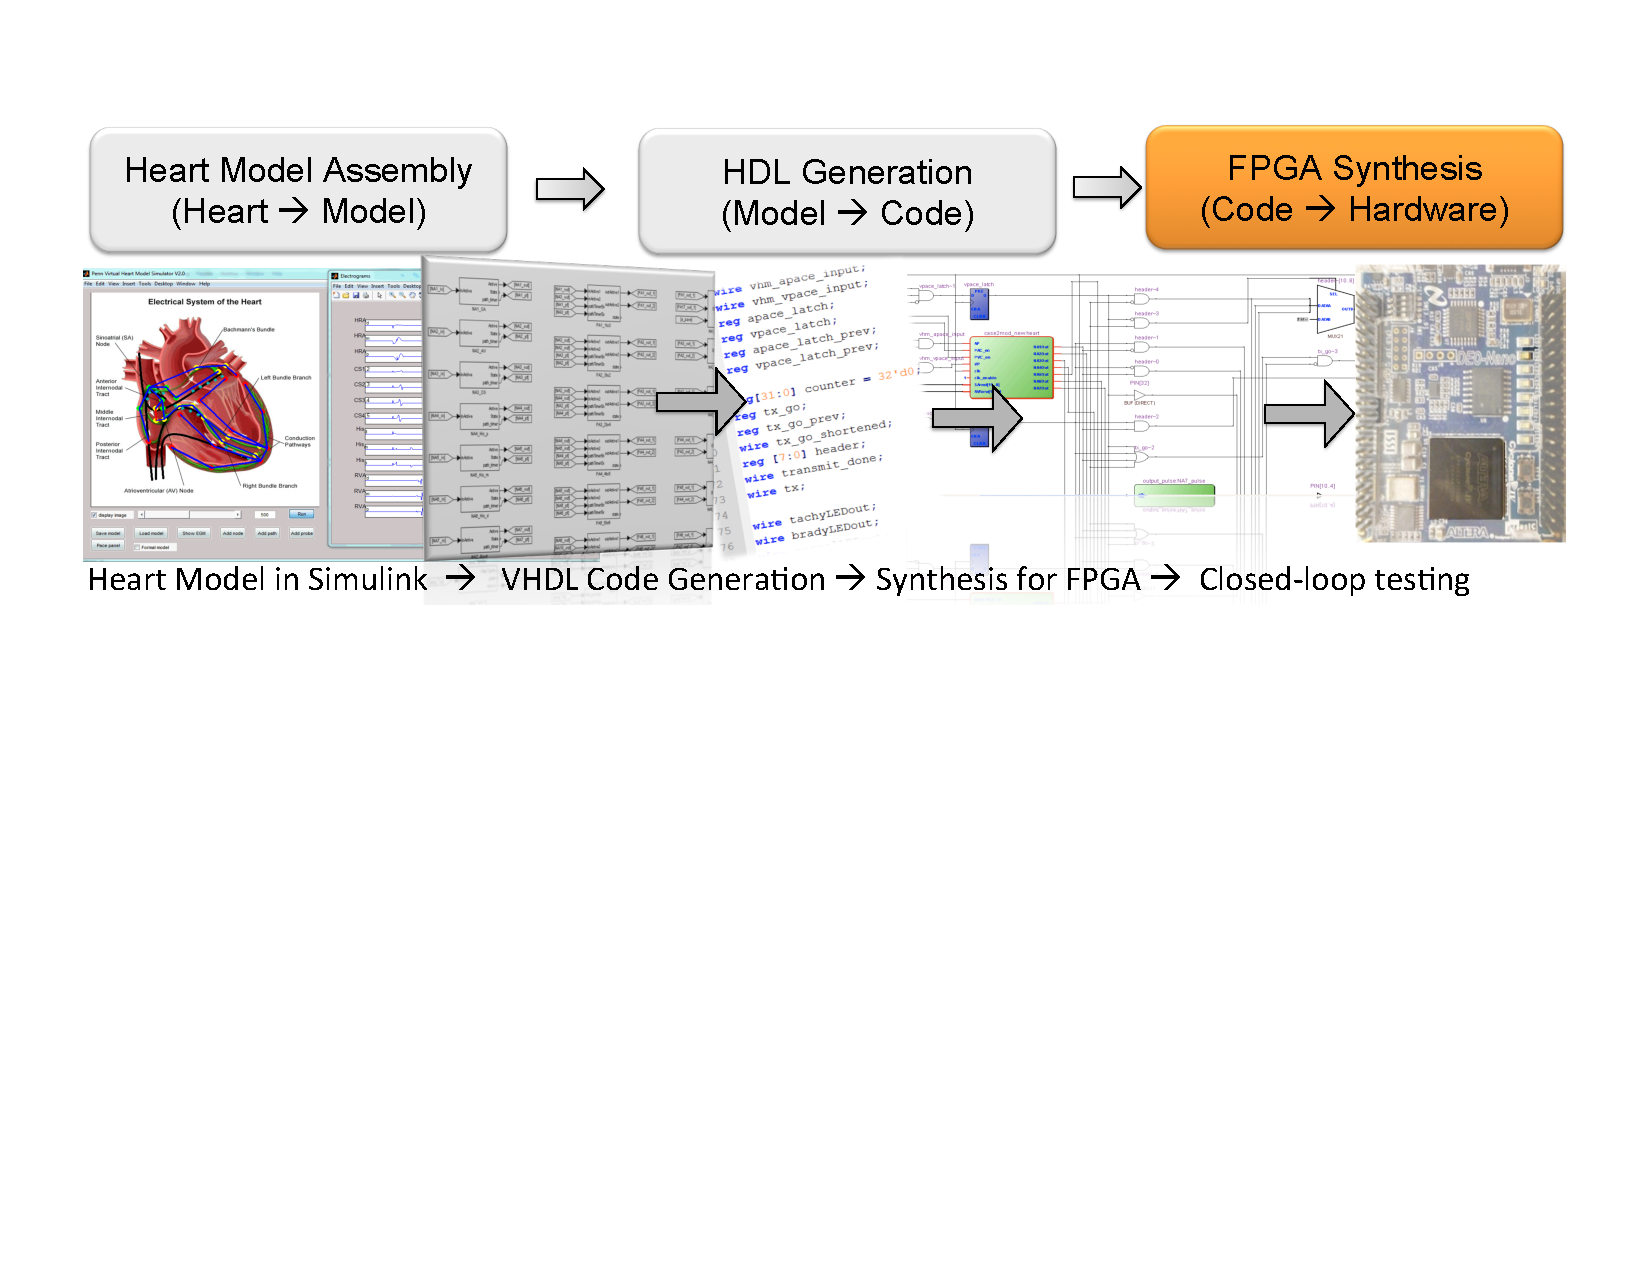
\includegraphics[width=0.98\textwidth]{figs/modeling_heart.pdf}
%\vspace{-10pt}
\caption{The heart model was developed in Matlab/Simulink and code was automatically generated to operate on an FPGA platform for platform-level testing.}
\label{fig:modeling_heart}
%\vspace{-15pt}
\end{figure}
\begin{figure}[!b]
\center
%\vspace{-15pt}
		\includegraphics[width=0.8\textwidth]{figs/PVS.pdf}
%\vspace{-10pt}
\caption{Heart-on-a-Chip testbed for real-time closed-loop testing of the pacemaker or model of the pacemaker with the heart model on the hardware platform}
\label{fig:HOC}
%\vspace{-15pt}
\end{figure}
\section{Heart Models for Closed-loop Model Checking}
%\begin{itemize}
	%\item What does nondeterminism do? Where can these model be used?
    %\item How to replace complex dynamics of the deterministic models with nondeterminism?
    %\item What are the abstraction rules that can be applied to the heart models and what are their physiological basis?
    %\item How to encode the information loss during each abstraction steps?
%\end{itemize}
During closed-loop model checking, the whole closed-loop state space of the device and the environment is mathematically explored against physiological requirements. The  ideal environment models should be: (1) simple enough to avoid the state space explosion problem (\cite{Abstraction}), (2) general enough to cover possible physiological operation parameters, and (3) expressive enough to represent specific physiological conditions in-depth. It is obvious that no single model can achieve all three properties. A rigorous framework should be adapted so that models with the appropriate level of refinement, from a family of models, are selected based on the requirement type. For example, for a simple property that the pacemaker must maintain the heart rate above a desired level, a relatively abstract model will suffice. For a more complex property such as the termination of Pacemaker Mediated Tachycardia (\cite{josephson}), an appropriately refined model which expresses the physiological condition will be selected.

\subsection{Modeling Philosophy}
\textbf{Model Formalism: }Choosing an appropriate formalism for the physiological models is important as the formalism determines the closed-loop state space and hence the feasibility to do model checking. The pacemaker utilizes the timing of local electrical events to diagnose heart conditions. It is therefore natural to use timed-automata models of the heart. With this formalism, we use the UPPAAL model checking tool (\cite{uppaal_tut}) such that the whole closed-loop state space is explored symbolically.\\\\
\textbf{Model Coverage: } Pacemakers are designed to treat bradycardia by maintaining the appropriate heart rate when the intrinsic rate is low. However, at the same time, a pacemaker should not adversely affect other heart conditions such as supraventricular tachycardia (\cite{pacemakerrecalls}). Even for the same patient, the heart condition changes over time and must be addressable by the modeling effort. In order to achieve safety across all possible heart conditions, the heart models used during closed-loop verification should be able to cover all possible heart behaviors, more precisely, their mapping to pacemaker inputs. Over-approximation (\cite{CEGAR}) with non-determinism can be used to simplify model structure while covering larger variety of environmental behaviors. Techniques like model-checking can then be used to examine the whole closed-loop state space for property violations.\\\\ 
\textbf{Ambiguity due to Limited Sensing Capability: }The spatial sensing resolution of pacemakers is low, in terms of the number of sensing location (2-3 leads), as well as the information obtained from each sensing location (binary events with no analog morphology). Through the process of abstraction, if different heart conditions are able to generate exactly the same input sequence to the pacemaker, there will be ambiguities in concretizing abstract closed-loop executions. For certain conditional requirements, it is important to differentiate all possible concrete executions corresponding to an abstract execution. As the result, the heart model(s) should have the capability to differentiate these heart conditions when verifying certain properties. Thus, a single heart model will not suffice and a family of heart models are required.\\\\
\textbf{Information Loss during Abstraction: }While over-approximation achieves simplicity and coverage, it also inevitably introduces invalid behaviors (e.g. not clinically feasible or relevant) into the model which can cause false-negatives and false-positives during model checking. To solve this problem, refined models of the heart should be available which can resolve spurious counterexamples and eliminate invalid executions when necessary to avoid false-positives.

The most challenging aspect during closed-loop model checking is the abstraction and refinement of the environment model. In \cite{STTT13} we developed a series of heart model abstractions at various abstraction levels. The models are abstracted using abstraction rules derived from physiological knowledge, thus ensuring that each abstraction step covers more physiological conditions. The models in adjacent abstraction levels also satisfy \textsf{timed-simulation} relationship (\cite{simulation}) to ensure complete coverage in the more abstract model. In the remainder of this section, we briefly discuss this multi-scale modeling process and the domain knowledge used. The detailed abstraction and proof for simulation relationship can be found in \cite{STTT13}.

\subsection{Timed Automata and Timed Simulation}
Timed automata (\cite{timed_automata}) is an extension of a finite automaton with a finite set of real-valued clocks. It has been used for modeling and verifying systems which are triggered by events and have timing constraints between events.  UPPAAL is a standard tool for modeling and verification of real-time systems, based on networks of timed automata. The graphical and text-based interface makes modeling more intuitive. Requirements can be specified using Computational Tree Logic (CTL), as described in \cite{Clarke}, and violations can be visualized in the simulation environment.

\emph{The rest of this section describes the process of model abstraction and refinement where more abstract models cover more of the state space but can only prove simpler properties. As we refine models, they cover lesser state space but can prove more complex properties. The reader looking for a more intuitive understanding of the area may skip the detailed description in the rest of this chapter, during the first reading.}
\newpage
\subsubsection{Syntax of Timed Automata}
A timed automaton \textbf{G} is a tuple $\left\langle S,S_0,\Sigma,X,inv,E\right\rangle$, where

\begin{itemize}
	\item $S$ is a finite set of locations.
	\item $S_0\in S$ is the set of initial locations.
	\item $\Sigma$ is the set of events.
	\item $X$ is the set of clocks.
	\item $inv$ is the set of invariants for clock constraints at each location.
	\item $E$ is the set of edges. Each edge is a tuple $\left\langle s,\sigma,\Psi,\lambda,s'\right\rangle$ which consists of a source location $s$, an event $\sigma\in\Sigma$, clock constraints $\Psi$, $\lambda$ as a set of clocks to be reset and the target location $s'$.   
\end{itemize}

For the clock variables $X$, the clock constraints $\Psi\in\Psi^X$ can be inductively defined by $\Psi:=x\bot c\|\Psi_1\wedge\Psi_2$, where $\bot\in\{\leq,=,\geq\}$, and $c\in\mathbb{N}$.
\subsubsection{Semantics of Timed Automata}
A state of a timed automaton is a pair $\left\langle s,v\right\rangle$ which contains the location $s\in S$ and the valuation $v$ for all clocks. The set of all states is $\Omega$. For all $\lambda\in X$, $v[\lambda :=0]$ denotes the valuation which sets all clocks $x\in\lambda$ as zero and the rest of the clocks unchanged. For all $t\in \textbf{R}$, $v+t$ denotes the valuation which increase all the clock value by $t$. There are two kinds of transitions between states. The \textsf{discrete transition} happens when the condition of an edge has been met. So we have:
$$\left\langle s,\sigma,\Psi,\lambda,s'\right\rangle\in E,v\models \Psi,v[\lambda :=0]\models inv(s')$$
$$\Rightarrow (s,v)\xrightarrow{\sigma}(s',v[\lambda :=0])$$
The \textsf{timed transition} happens when the timed automaton can stay in the same location for certain amount of time. We have:
$$\delta\in \textsl{R},\forall \delta'\leq\delta, v+\delta'\models inv(s)$$
$$\Rightarrow (s,v)\xrightarrow{\delta}(s,v+\delta)$$
\subsubsection{Timed Simulation}
For two timed automata $T^1=\left\langle S^1,S_0^1,\Sigma^1,X^1,inv^1,E^1\right\rangle$ and $T^2=\left\langle S^2,S_0^2,\Sigma^2,X^2,inv^2,E^2\right\rangle$, a timed simulation relation is a binary relation $\textsf{sim}\subseteq \Omega^1\times \Omega^2$ where $\Omega^1$ and $\Omega^2$ are sets of states of $T^1$ and $T^2$. We say $T^2$ \textsf{time simulates} $T^1$ ($T^1 \preceq_t T^2$) if the following conditions holds:
\begin{itemize}
	\item Initial states correspondence: $(\left\langle s_0^1,\textbf{0}\right\rangle,\left\langle s_0^2,\textbf{0}\right\rangle)\in \textsf{sim}$
	\item Timed transition: For every $(\left\langle s_1,v_1\right\rangle,\left\langle s_2,v_2\right\rangle)\in\textsf{sim}$, if $\left\langle s_1,v_1\right\rangle\xrightarrow{\delta}\left\langle s_1,v_1+\delta\right\rangle$, there exists $\left\langle s_2,v_2+\delta\right\rangle$ such that $\left\langle s_2,v_2\right\rangle\xrightarrow{\delta}\left\langle s_2,v_2+\delta\right\rangle$ and \\$(\left\langle s_1,v_1+\delta\right\rangle,\left\langle s_2,v_2+\delta\right\rangle)\in\textsf{sim}$.
	\item Discrete transition: For every $(\left\langle s_1,v_1\right\rangle,\left\langle s_2,v_2\right\rangle)\in\textsf{sim}$, if $\left\langle s_1,v_1\right\rangle\xrightarrow{\sigma}\left\langle s_1',v_1'\right\rangle$, there exists $\left\langle s_2',v_2'\right\rangle$ such that $\left\langle s_2,v_2\right\rangle\xrightarrow{\sigma}\left\langle s_2',v_2'\right\rangle$ and $(\left\langle s_1',v_1'\right\rangle,\left\langle s_2',v_2'\right\rangle)\in\textsf{sim}$.
\end{itemize}

Certain properties are preserved for timed simulation relation. For $\varphi\in ATCTL$, if $M\preceq_t M'$, we have $M'\models \varphi\Rightarrow M\models\varphi$.\cite{simulation} However, $M'\not\models \varphi\Rightarrow M\not\models\varphi$ does not hold. Violations of $ATCTL$ yield \textsf{counter-examples} and the validity of which need to be checked on more refined model.

\begin{figure}[!t]
\center
%\vspace{-10pt}
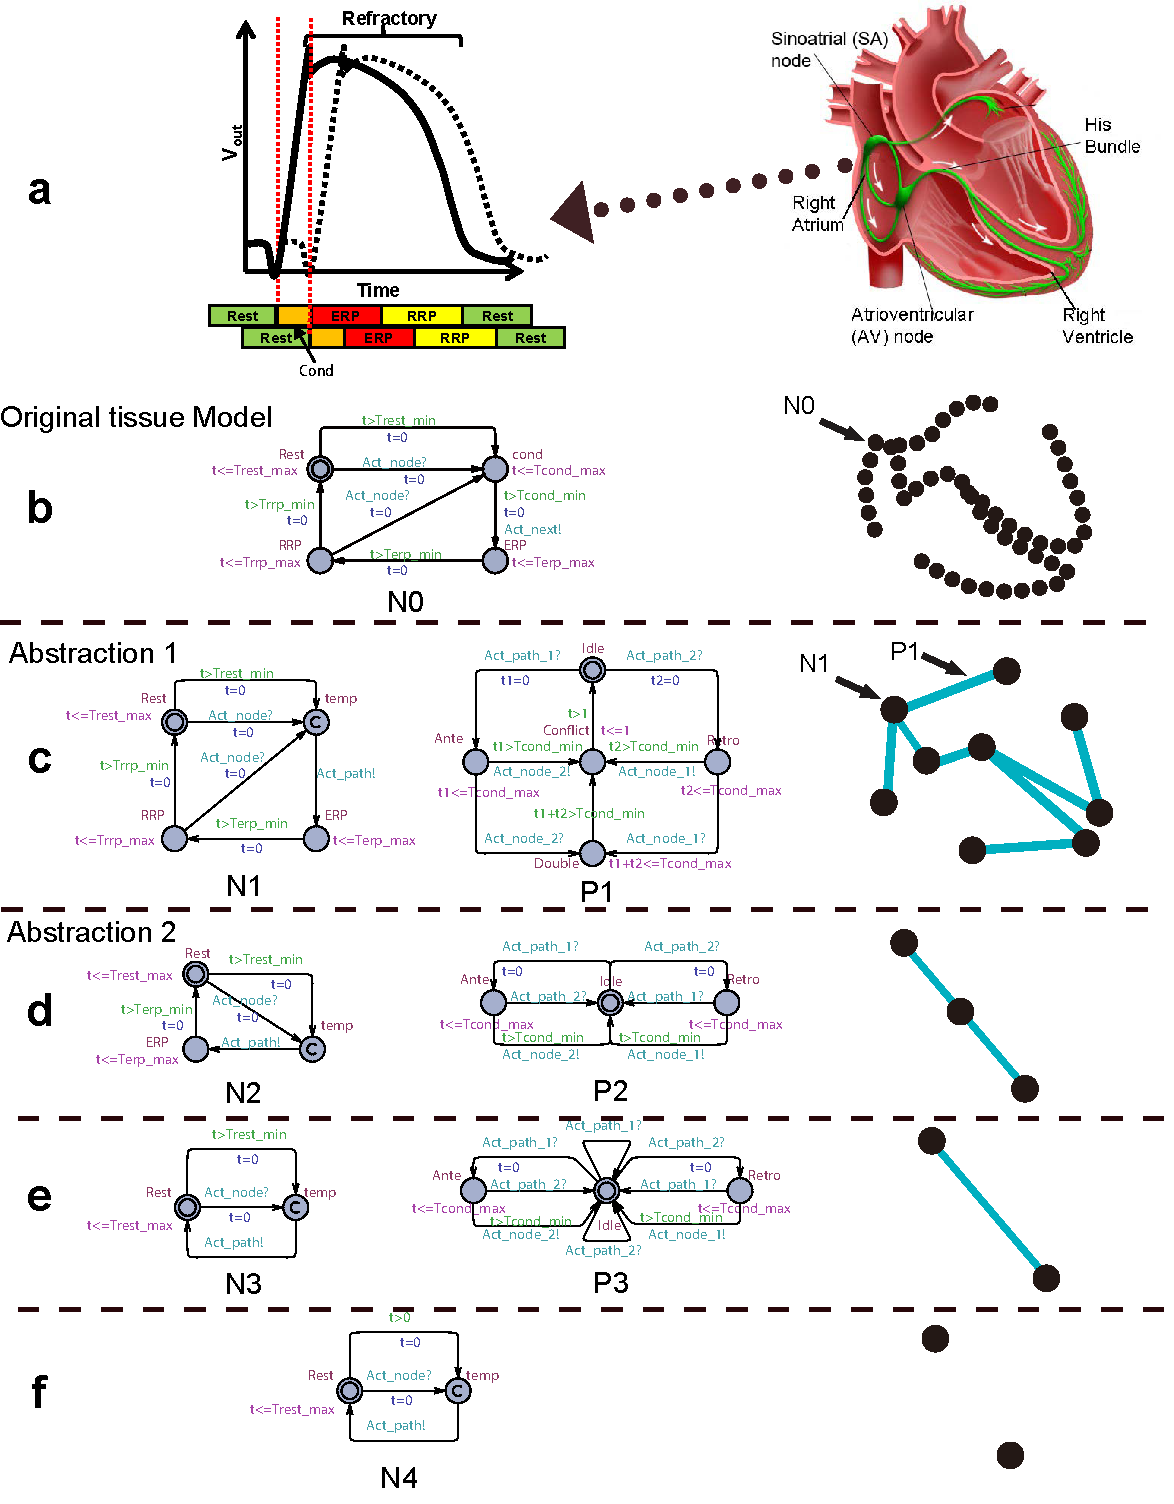
\includegraphics[width=\textwidth]{figs/Heart_abs.pdf}
%\vspace{-10pt}
\caption{(a) Electrical voltage change measured on the heart tissue and its adjacent tissue region (dotted) upon activation. The whole process is divided into timing periods with different behaviors. (b) The original tissue model which captures the refactory timing behaviors of the heart tissue. (c) The conduction property is separated to the path automaton and the heart can be modeled as conduction network. (d) Equivalent locations are merged. (e) The blocking property of the ERP location is replaced by a non-deterministic conduction in the path automaton. (f) Conduction between nodes are replaced by self-activations of the nodes. More details in \cite{STTT13}}
\label{fig:HM_abs}
\vspace{-10pt}
\end{figure} 
It is known that timed simulation relation is also closed under composition \cite{simulation}. So when we have two heart models $H_1\preceq_t H_2$ we will have $H_1\| P\preceq_t H_2\| P$ where $P$ is the timed-automata model of the pacemaker. For $\varphi\in ATCTL$, we have $H_2\| P\models\varphi\Rightarrow H_1\| P\models\varphi$. With this property we can verify the pacemaker model with abstract heart model. In the rest of the section, we will describe how we develop our initial heart model from the physiological perspective and abstract the model step by step so that the complexity of the model is reduced for verification. Given two heart models $H_1$, $H_2$ and a timed simulation mapping \textsf{sim}=$\Omega_1\times\Omega_2$, there are no automated methods to check $H_1\preceq_t H_2$. In the Appendix, we show the manual proof for the timed simulation relation between two heart models $H_2$ and $H_3$. Other timed simulation relations can be proved similarly.

\subsection{Abstraction 0: Initial Abstraction}
For the initial heart model, we assume the heart tissue is modeled with all its spatial detail. For the temporal aspect, we model each tissue region as an automaton $N0$ shown in \figref{HM_abs}(b). The beat-to-beat dynamics of heart tissue, modeled by the deterministic model, is abstracted using non-determinism. For example, the ERP period and conduction delay of the tissue are non-deterministically chosen from ranges instead of deterministic functions. The whole heart can be modeled by composing tissue models with different parameters $H_0=N_0^1\|N_0^2\cdots N_0^n$. However, for a real heart, the number $n$ is very large and the connectivity and parameter values are difficult, and perhaps impossible, to determine, which makes verification with $H_0$ infeasible. 

\subsection{Abstraction 1: Abstract Conduction Delays With Paths}
At the first abstraction step, we separate the conduction delay (modeled by the \emph{cond} state in $N0$) from the new node automata $N1$ and model the conduction between two nodes using path automaton $P1$. Since the beat-to-beat dynamics are abstracted with non-determinism, the RRP state is merged with the Rest state in $N1$. The procedure gives us the intuition to abstract the heart as a conduction network as shown in \figref{HM_abs} (c). 

\subsection{Abstraction 2: Merging Equivalent States}
The heart model $H_1'$ still has equivalent locations. In Abstraction 2 we further abstract the node and path automata by merging equivalent states. In the new node automaton $N_2$ we merge the \textsf{RRP} state with the \textsf{Rest} state with:
$$N_2.Trest\_min = N_1.Trest\_min+N_1.Trrp\_min$$
$$N_2.Trest\_max = N_1.Trest\_max+N_1.Trrp\_max$$
Under the assumption that the ERP period of a node automaton is much longer than the conduction delay of a path automaton,  the \textsf{Double} and \textsf{Conflict} location of the path automaton is merged with the \textsf{Idle} state. The heart can be modeled as $H_2=N_2^1\| P_2^1\| N_2^2\| P_2^2\| N_2^3$.

\subsection{Abstraction 3: Replacing Blocking with Non-deterministic Conduction}
In Abstraction 3, we replace the blocking behavior of the \textsf{ERP} location of the node with non-deterministic conduction in the path automaton. There exists a transition\\ 
$$RE\| ID\| RE \xrightarrow[Act\_path\_1!]{Act\_node\_1?}\xrightarrow{Act\_path\_1?}RE\| ID\| RE$$
in $N_3^1\| P_3^1\| N_3^2$ to replace transition\\
$$ER\| ID\| ER \xrightarrow{Act\_node\_1?} ER\| ID\| ER$$
in $N_2^1\| P_2^1\| N_2^2$

Without the ERP constraint the AV node is no longer needed and the heart can be modeled as $H_3=N_3^1\| P_3\| N_3^2$.  The detailed proof for this timed simulation relation can be found in \cite{STTT13}. 
\subsection{Abstraction 4: Random Heart Model (RHM)}
In Abstraction 4, we further simplify the heart model by removing the conduction path between two nodes. By setting $Trest\_min$ for both nodes to 0 the new heart model $H_4=N_3^1\|N_3^2$ covers all possible behavior of $H_3$. This random heart model with two nodes is the most abstract model that will be used at the beginning of the closed-loop model checking process.
%\textbf{AG}$\varphi\equiv\neg$\textbf{EF}($\neg\varphi$) 

Eventually we have a series of heart models with:

$N_0^1\|N_0^2\cdots N_0^n$\\
$\preceq_t N_1^1\|P_1^1\|N_1^2\cdots P_1^{m}\|N_1^n$\\
$\preceq_t N_1^1\| P_1^1 \| N_1^2\| P_1^2 \| N_1^3$\\
$\preceq_t N_2^1\| P_2^1\| N_2^2\| P_2^2\| N_2^2$\\
$\preceq_t N_3^1\| P_3\| N_3^2$\\
$\preceq_t N_4^1\| N_4^2$

Using this technique, we systematically create a family of heart models with different levels of complexity and expressiveness. In Chapter \ref{ModelChecking} we describe how to balance between complexity and expressiveness and use these heart models for closed-loop model checking of implantable pacemaker.
% \subsubsection{Abstracting Beat-to-beat Dynamics}
% \subsubsection{Abstracting Conduction Delays with Path}
% \subsubsection{Merging Activation-generating Nodes}
% \subsubsection{Replace ERP Blocking With Non-deterministic Conduction}
% \subsubsection{Replace }

\subsection{Discussion}
In this chapter, we use heart modeling as example to demonstrate how to develop physiological models for closed-loop evaluation of closed-loop medical devices. We emphasized that models should be developed according to their applications. We developed heart models based on clinical Electrophysiological Testing, and modeled the topological and temporal behaviors of the heart with timed-automata formulation. In the next chapter we will demonstrate the identification and validation of the heart models.


